\documentclass[12pt]{extreport} % Schriftgröße: 8pt, 9pt, 10pt, 11pt, 12pt, 14pt, 17pt oder 20pt


%% Packages
\usepackage{scrextend}
\usepackage{amssymb}
\usepackage{amsthm}
\usepackage{booktabs}
\usepackage{chngcntr}
\usepackage{cmap}
\usepackage{color}
\usepackage{enumerate}
\usepackage{float}
\usepackage{hyperref}
\usepackage{ulem}
\usepackage{lmodern}
\usepackage{makeidx}
\usepackage{mathtools}
\usepackage{xpatch}
\usepackage{pgfplots}
\usepackage{stackengine}
\pgfplotsset{compat=1.7}
\usetikzlibrary{calc}	
\usetikzlibrary{matrix}	

% Language Setup (Deutsch)
\usepackage[utf8]{inputenc} 
\usepackage[T1]{fontenc} 
\usepackage[ngerman]{babel}

\usepackage{csquotes}
% Options
\makeatletter%%  
  % Publisher definieren
  \newcommand\publishers[1]{\newcommand\@publishers{#1}} 
  % Enumerate im 1. Level: \alph für a), b), ...
  \renewcommand{\labelenumi}{\alph{enumi})} 
  % Enumerate im 2. Level: \roman für (i), (ii), ...
  \renewcommand{\labelenumii}{(\roman{enumii})}
  % Zeileneinrückung am Anfang des Absatzes
  \setlength{\parindent}{0pt} 
  % Für das Proof-Environment: 'Beweis:' anstatt 'Beweis.'
  \xpatchcmd{\proof}{\@addpunct{.}}{\@addpunct{:}}{}{} 
  % Nummerierung der Bilder, z.B.: Abbildung 4.1
  \@ifundefined{thechapter}{}{\def\thefigure{\thechapter.\arabic{figure}}} 
\makeatother%

% Meta Setup (Für Titelblatt und Metadaten im PDF)
\title{Globale Optimierung}
\author{Prof. Dr. Oliver Stein}
\date{Sommersemester 2017}
\publishers{Karlsruher Institut für Technologie}

%% Math. Definitionen
\newcommand{\C}{\mathbb{C}}
\newcommand{\N}{\mathbb{N}}
\newcommand{\Q}{\mathbb{Q}}
\newcommand{\R}{\mathbb{R}}
\newcommand{\Z}{\mathbb{Z}}
\renewcommand*{\qed}{\hfill\ensuremath{\square}}

\theoremstyle{named}
\newtheorem{unnamedtheorem}{Theorem} 
\theoremstyle{nnamed}
\newtheorem*{unnamedtheorem*}{Theorem} 

\theoremstyle{itshape}
\newtheorem*{satz}{Satz} 
\newtheorem*{definition}{Definition}
\newtheorem*{hilfssatz}{Hilfssatz}

\theoremstyle{normal}
\newtheorem*{anwendung}{Anwendung}
\newtheorem*{beispiels}{Beispiel}
\newtheorem*{bemerkung}{Bemerkung} 
\newtheorem*{bezeichnung}{Bezeichnung}
\newtheorem*{eigenschaft}{Eigenschaft}
\newtheorem*{erinnerung}{Erinnerung}
\newtheorem*{folgerung}{Folgerung}
\newtheorem*{korollar}{Korollar}
\newtheorem*{lemma}{Lemma}
\newtheorem*{motivation}{Motivation}
\newtheorem*{uebung}{Übung}
\newtheorem*{vereinbarung}{Vereinbarung}

\makeatletter%
\DeclareUnicodeCharacter{00A0}{ } \pgfplotsset{compat=1.7} \hypersetup{colorlinks,breaklinks, urlcolor=linkcolor, linkcolor=linkcolor, pdftitle=\@title, pdfauthor=\@author, pdfsubject=\@title, pdfcreator=\@publishers}
\DeclareOption*{\PassOptionsToClass{\CurrentOption}{report}} 
\ProcessOptions 
\def\baselinestretch{1.25} \setlength{\oddsidemargin}{0.125in} \setlength{\evensidemargin}{0.125in} \setlength{\topmargin}{0.5in} \setlength{\textwidth}{6.25in} \setlength{\textheight}{8in} \addtolength{\topmargin}{-\headheight} \addtolength{\topmargin}{-\headsep} \def\pulldownheader{ \addtolength{\topmargin}{\headheight} \addtolength{\topmargin}{\headsep} \addtolength{\textheight}{-\headheight} \addtolength{\textheight}{-\headsep} } \def\pullupfooter{ \addtolength{\textheight}{-\footskip} } \def\ps@headings{\let\@mkboth\markboth \def\@oddfoot{} \def\@evenfoot{} \def\@oddhead{\hbox {}\sl \rightmark \hfil \rm\thepage} \def\chaptermark##1{\markright {\uppercase{\ifnum \c@secnumdepth >\m@ne \@chapapp\ \thechapter. \ \fi ##1}}} \pulldownheader } \def\ps@myheadings{\let\@mkboth\@gobbletwo \def\@oddfoot{} \def\@evenfoot{} \def\sectionmark##1{} \def\subsectionmark##1{}  \def\@evenhead{\rm \thepage\hfil\sl\leftmark\hbox {}} \def\@oddhead{\hbox{}\sl\rightmark \hfil \rm\thepage} \pulldownheader }	\def\chapter{\cleardoublepage  \thispagestyle{plain} \global\@topnum\z@ \@afterindentfalse \secdef\@chapter\@schapter} 
\def\@makeschapterhead#1{ {\parindent \z@ \raggedright \normalfont \interlinepenalty\@M \Huge \bfseries  #1\par\nobreak \vskip 40\p@ }} \newcommand{\indexsection}{chapter} \patchcmd{\@makechapterhead}{\vspace*{50\p@}}{}{}{}\def\Xint#1{\mathchoice
    {\XXint\displaystyle\textstyle{#1}} {\XXint\textstyle\scriptstyle{#1}} {\XXint\scriptstyle\scriptscriptstyle{#1}} {\XXint\scriptscriptstyle\scriptscriptstyle{#1}} \!\int} \def\XXint#1#2#3{{\setbox0=\hbox{$#1{#2#3}{\int}$} \vcenter{\hbox{$#2#3$}}\kern-.5\wd0}} \def\dashint{\Xint-} \def\Yint#1{\mathchoice {\YYint\displaystyle\textstyle{#1}} {\YYYint\textstyle\scriptscriptstyle{#1}} {}{} \!\int} \def\YYint#1#2#3{{\setbox0=\hbox{$#1{#2#3}{\int}$} \lower1ex\hbox{$#2#3$}\kern-.46\wd0}} \def\YYYint#1#2#3{{\setbox0=\hbox{$#1{#2#3}{\int}$}  \lower0.35ex\hbox{$#2#3$}\kern-.48\wd0}} \def\lowdashint{\Yint-} \def\Zint#1{\mathchoice {\ZZint\displaystyle\textstyle{#1}}{\ZZZint\textstyle\scriptscriptstyle{#1}} {}{} \!\int} \def\ZZint#1#2#3{{\setbox0=\hbox{$#1{#2#3}{\int}$}\raise1.15ex\hbox{$#2#3$}\kern-.57\wd0}} \def\ZZZint#1#2#3{{\setbox0=\hbox{$#1{#2#3}{\int}$} \raise0.85ex\hbox{$#2#3$}\kern-.53\wd0}} \def\highdashint{\Zint-} \DeclareRobustCommand*{\onlyattoc}[1]{} \newcommand*{\activateonlyattoc}{ \DeclareRobustCommand*{\onlyattoc}[1]{##1} } \AtBeginDocument{\addtocontents{toc} {\protect\activateonlyattoc}} 
	% Titlepage
	\def\maketitle{ \begin{titlepage} 
			~\vspace{3cm} 
		\begin{center} {\Huge \@title} \end{center} 
	 		\vspace*{1cm} 
	 	\begin{center} {\large \@author} \end{center} 
	 	\vspace*{-0.5cm}
	 	\begin{center} \@date \end{center} 
	 		\vspace*{7cm} 
	 	\begin{center} \@publishers \end{center} 
	 		\vfill 
	\end{titlepage} }
\usepackage{filecontents}
\begin{filecontents*}{MyPackage.sty}
\NeedsTeXFormat{LaTeX2e}
\ProvidesPackage{MyPackage}
\RequirePackage{environ}
\newif\if@hidden% \@hiddenfalse
\DeclareOption{hide}{\global\@hiddentrue}
\ProcessOptions\relax
\NewEnviron{beispiel}
  {\if@hidden\else\begin{beispiels}\BODY\end{beispiels}\fi}
\end{filecontents*}
\usepackage[hide]{MyPackage}
\makeatother%


% Create Index
\makeindex 

\begin{document}

\thispagestyle{empty}

\pagenumbering{Alph}
\begin{titlepage}
	\maketitle
	\thispagestyle{empty}
\end{titlepage}

% Skript - Anfang 			
\pagenumbering{arabic}

% todo online fragen

\chapter{Einführungen}

\section{Grundbegriffe}

Zwei grundlegende Begriffe in der Optimierung sind der \textbf{optimale Punkt} und der \textbf{optimale Wert}. Als Beispiel kann man fragen, wer in einer Gruppe von Personen die meisten Münzen bei sich trägt. Der optimale Wert ist die gefundene größtmögliche Anzahl von Münzen. Er ist eindeutig bestimmt. Im Gegensatz dazu können durchaus mehrere Personen diese Anzahl von Münzen bei sich tragen. Demnach ist der Punkt (hier: die Person), an dem der optimale Wert angenommen wird, nicht notwendigerweise eindeutig. Dies gilt analog bei jedem Optimierungsproblem.

\begin{beispiel}[Projektion auf eine Menge] ~\\
Sei $M \subseteq \R^n$ und $z \in \R^n$
$$ P_M: \quad \min_{x \in \R^n} \| x - z \|_2 \text{ s.t. } x \in M. $$
Nach Satz 1.2.10 ist dieses Projektionsproblem für jede nicht-leere und kompakte Menge $M \subseteq \R^n$ lösbar, denn $\| \cdot \|_2$ ist eine stetige Funktion. ~\\

\textit{Beachte: Projektion unter euklidischer Norm = orthogonale Projektion} ~\\

Falls $M$ eine Hyperebene ist, lässt sich das Problem $P_M$ explizit lösen. Dazu sei 
$$ M = \left\{ x \in \R^n \colon a^T x = b \right\}, $$
d.h. $M$ sei durch eine lineare Gleichung beschrieben. Dann wird das Optimierungsproblem $P$ zu
$$ P_M\colon \min_{x \in \R^n} \| x - z \|_2 \text{ s.t. } a^Tx = b $$
damit ist der eindeutige optimale Punkt $\overline{x}$ und der dazugehörige optimale Wert $v$ gegeben durch
$$ \overline{x} = z - \frac{a^T z - b}{a^T a} \cdot a, ~ v = \left| \frac{a^T z - b}{a^T a} \cdot a \right|_2 = \frac{\left| a^T z - b \right|}{\| a \|_2}$$
\end{beispiel}


\begin{definition}[Minimalpunkte und Minimalwerte] ~\\
	Gegeben sei eine Menge von zulässigen Punkte $M \subseteq \R$ und eine Zielfunktion $f \colon M \rightarrow \R$.
	\begin{enumerate}
		\item $\overline{x} \in M$ heißt \textbf{lokaler Minimalpunkt} von $f$ auf $M$, falls eine Umgebung $U$ von $\overline{x}$  existiert mit
			$$ \forall x \in U \cap M: \quad f(x) \geq f(\overline{x}). $$
		\item $\overline{x} \in M$ heißt \textbf{globaler Minimalpunkt} von $f$ auf $M$, falls man in a) $U = \R^n$ wählen kann.
		\item Ein lokaler oder globaler Minimalpunkt heißt \textbf{strikt}, falls in a) bzw. b) für $x \neq \overline{x}$ sogar die strikte Ungleichung \enquote{$>$} gilt.
		\item Zu jedem globalen Minimalpunkt $\overline{x}$ heißt $f(\overline{x})$ ($= v = \min_{x \in M} f(x)$) \textbf{globaler}, und zu jedem lokalen Minimalpunkt $\overline{x}$ heißt $f(\overline{x})$ \textbf{lokaler Minimalwert}.
	\end{enumerate}
	Strikte globale Minimalpunkte sind eindeutig, und strikte lokale Minimalpunkte sind lokal eindeutig.
\end{definition}

\begin{beispiel}[1.1.5, 1.2.26, 1.2.31 Zentrum einer Punktewolke] ~\\
	Gegeben seien Punkte $x^1, x^2, \dotsc, x^m \in \R^n$. Gesucht ist ein Punkt $z \in \R^n$ \enquote{im Zentrum der Punkte}. Benutzt man die 2-Norm so führt dies auf das Optimierungsproblem
		$$ P: \quad \min_{z \in \R^n} \left\| \left( \| z - x^2 \|_2, \dotsc \| z - x^m \|_2 \right)^T \right\|_2, $$
	ohne Nebenbedingungen. Als Optimalpunkt berechnet man das arithmetische Mittel der Punkte
	$$ \overline{z} = \frac{1}{m} \sum_{i=1}^m x^i. $$
	Ein Problem dieses Ansatzes besteht darin, dass Ausreißer bei wachsender Punkteanzahl $m$ vernachlässigt werden. Eine Möglichkeit dieses Problem zum umgehen, könnte 
	$$ \| x \|_\infty = \max_{j=1, \dotsc, n} |x_j| $$ 
	als äußere Norm zu verwenden. ~\\
	
	Dieses Problem ist koerziv, denn es gilt
	$$ f(z) = \sqrt{\sum_{i=1}^m \| z - x^i \|_2^2} \geq \sqrt{\| z - x^1 \|_2^2} = \| z - x^1 \| \geq \left| \| z \| - \| x^1 \|_2 \right| \xrightarrow[\| z\|\rightarrow \infty]{} +\infty $$
	Somit ist dieses Beispiel nach 1.2.26 und Korollar 1.2.30 lösbar.
\end{beispiel}

\begin{definition}[Epigraph]
	Für $M \subseteq \R^n$ und $f \colon M \rightarrow \R$ heißt die Menge
	$$ \operatorname{epi}(f, M) = \big\{ (x, \alpha) \in M \times \R ~|~ f(x) \leq \alpha \big\} $$
	\textbf{Epigraph} von $f$ auf $M$. Der Epigraph besteht aus dem Graphen von $f$ auf $M$ sowie allen darüber liegenden Punkten.
\end{definition}

Die Suche nach einem Minimalpunkt von $f$ auf $m$ ist äquivalent zur Suche nach einem $(x, \alpha)$ mit minimaler $\alpha$-Komponente auf dem Epigraphen von $f$ (vgl. Übung 1.3.7). % todo Uebung

\begin{definition}[Epigraph-Umformulierung]
	Das Problem 
		$$ P: \quad \min_x f(x) \text{ s.t. } x \in M $$
	ist in diesem Sinne also äquivalent zu
		$$ P_{epi}: \quad \min_{(x, \alpha)} \alpha \text{ s.t. } f(x) \leq \alpha, ~x \in M. $$
\end{definition}

\begin{beispiel}[Epigraph-Umformulierung der Punktewolke] ~\\
	Im vorliegenden Fall des Zentrums einer Punktwolke mit Maximumsnorm als äußerer Norm gilt
		$$ P: \quad \min_{z \in \R^n} \left\| \left( \| z - x^2 \|_2, \dotsc \| z - x^m \|_2 \right)^T \right\|_2, $$
	also $M = \R^n$ und 
		$$ f(z) = \max_{i=1, \dotsc, m} \| z - x^i \|_2. $$
	Die Epigraph-Umformulierung lautet dann
		$$ P_{epi}: \quad \min_{(z, \alpha)} \alpha \text{ s.t. } f(z) \leq \alpha, $$
	wobei die Nebenbedingung von $P_{epi}$ ausgeschrieben lautet:
	$$ \max_{i=1, \dotsc, m} \| z - x^i \|_2 \leq \alpha; $$
	bzw. das Maximum ausnutzend:
	$$ P_{epi}: \quad \min_{(z, \alpha)} \alpha \text{ s.t. } \| z - x^i \|_2 \leq \alpha, ~ i = 1, \dotsc, m $$
	d.h. man sucht einen Kreis mit Mittelpunkt $z$ und minimalem Radius $\alpha$ zu finden, der alle Punkte $x^1, \dotsc, x^m$ enthält.
\end{beispiel}

\begin{beispiel}[1.1.6, 1.2.27, Clusteranalyse]
	Anstatt wie bei der Punktewolke nur nach einem Mittelpunkt zu suchen, gehen wir nun von $k$ Zentren aus. Das Problem ergibt sich dann zu
	$$ P: \quad \min_{z^1, \dotsc, z^k \in \R^n} \left\| \left( \min_{\ell = 1, \dotsc, k} \| z^{\ell} - x^1 \|, \dotsc, \min_{\ell = 1, \dotsc, k} \| z^\ell - x^m \| \right)^T \right\| $$ 
	Als äußere Norm benutzt man häufig die $\ell_1$-Norm, d.h.
	$$ P_1: \quad \min_{z^1, \dotsc, z^k \in \R^n} \sum_{i=1}^{m} \min_{\ell = 1, \dotsc, k} \| z^\ell - x^i \| $$
	oder auch die $\ell_\infty$-Norm mit
	$$ P_\infty: \quad \min_{z^1, \dotsc, z^k \in \R^n} \max_{i=1, \dotsc, m} \min_{\ell = 1, \dotsc, k} \| z^\ell - x^i \|. $$	
	Beachte: der Vektor der Entscheidungsvariable im Problem hat in jedem Fall die Dimension $n \cdot k$, so dass in praktisch relevanten Anwendungen häufig hochdimensionale Probleme auftreten. Dieses Problem ist nicht koerziv.
\end{beispiel}

\newpage

\section{Lösbarkeit}

\begin{definition}[Infimum]
	Wir bezeichnen mit $\alpha \in \R$ die \textbf{untere Schranke} für $f$ auf $M$, falls
	$$ \forall x \in M: \quad \alpha \leq f(x) $$
	gilt. Das \textbf{Infimum} von $f$ auf $M$ ist die größte untere Schranke von $f$ auf $M$, es gilt also $v = \inf_{x \in M} f(x)$ falls
	\begin{itemize}
		\item $\forall x \in M$: $v \leq f(x)$ (d.h. $v$ ist selbst untere Schranke) und
		\item für alle unteren Schranken $\alpha$ von $f$ auf $M$ als kleinste obere Schranke definiert.
	\end{itemize}
	Analog wird das \textbf{Supremum} $\sup_{x \in M} f(x)$ von $f$ auf $M$ als kleinste obere Schranke definiert. ~\\
	
	Falls $f$ auf $M$ nicht nach unten beschränkt ist, setzt man formal
	$$ \inf_{x \in M} f(x) = - \infty, $$
	und für das Infimum über die leere Menge definiert man formal
	$$ \inf_{x \in \emptyset} f(x) = +\infty. $$
\end{definition}

\begin{definition}[1.2.3, Lösbarkeit]
	Das Minimierungsproblem $P$ heißt \textbf{lösbar}, falls ein $\overline{x} \in M$ mit $\inf_{x \in M} f(x) = f(\overline{x})$ existiert. ~\\
	
	Um anzudeuten, dass das Infimum angenommen wird, schreiben wir $\min_{x \in M} f(x)$ anstelle von $\inf_{x \in M} f(x)$.
\end{definition}

\begin{satz}[1.2.5]
	Das Minimierungsproblem $P$ ist genau dann lösbar, wenn es einen globalen Minimalpunkt besitzt.
\end{satz}

\newpage

\section{Arten von Unlösbarkeit}

\begin{definition}[1.2.6]
	Wir bezeichnen mit $\operatorname{pr}(z, M)$ die Menge der \textbf{orthogonalen Projektionen} eines Punktes $z \in \R^n$ auf $M \subseteq \R^n$ und mit
	$$ \operatorname{pr}(Z, M) = \big\{ \operatorname{pr}(z, M) ~|~ z \in M \big\} $$
	die orthogonale Projektion einer Menge $Z \subseteq \R^n$ auf $M$.
\end{definition}

\begin{definition}[1.2.7, Parallelprojektion]
	Für $Z \subseteq \R^n = R^k \times R^\ell$ heißt
	$$ \operatorname{pr}_a(Z) = \big\{ a \in \R^k ~|~\exists b \in \R^\ell \colon (a, b) \in Z \big\}. $$
	\textbf{Parallelprojektion} von $Z$ in die Menge $\R^k$.
\end{definition}

\begin{folgerung}[Parallelprojektion der Epigraphen]
	Die Parallelprojektion von $\operatorname{epi}(f, M)$ auf den \enquote{$\alpha$-Raum} $\R$ lautet also
	$$ \operatorname{pr}_\alpha \operatorname{epi}(f, M) = \big\{ \alpha \in \R ~|~\exists x \in M: f(x) \leq \alpha \big\} $$
\end{folgerung}

\begin{satz}[1.2.8]
	Für jedes Optimierungsproblem $P$ hat die Menge $\operatorname{pr}_{\alpha} \operatorname{epi}(f, M)$ genau eine der vier Gestalten
	\begin{enumerate}
		\item $\operatorname{pr}_{\alpha} \operatorname{epi}(f, M) = \emptyset$
		\item $\operatorname{pr}_{\alpha} \operatorname{epi}(f, M) = \R$
		\item $\operatorname{pr}_{\alpha} \operatorname{epi}(f, M) = (v, +\infty)$ mit $v \in \R$
		\item $\operatorname{pr}_{\alpha} \operatorname{epi}(f, M) = [v, +\infty)$ mit $v \in \R$
	\end{enumerate}
	Ferner ist der Fall a) zu $M =\emptyset$ % todo missing
\end{satz}

\begin{beispiel}[Distanz eines Punktes von einer Menge]
	Für eine Menge $M \subseteq \R^n$ und einen Punkt $z \in \R^n$ heißt
	$$ \operatorname{dist}(z, M) \coloneqq \inf_{x \in M} \| x - z \|_2 $$	
	Distanz von $z$ zu $M$. Wegen der Nichtnegativität der Norm ist Unlösbarkeit wegen Unbeschränktheit für dieses Problem nicht möglich. Ferner gilt 
	$$ \operatorname{dist}(z, \emptyset) = +\infty \text{ für jedes } z \in \R^n. $$
	Beachte: die fehlende Abgeschlossenheit von $M$ führt hier zu Unlösbarkeit.
\end{beispiel}

\newpage

\section{Der Satz von Weierstraß}

Eine Minimalvoraussetzung für die Lösbarkeit ist offensichtlich die Konsistenz von $M$, also $M \neq \emptyset$.

\begin{satz}[1.2.10, Satz von Weierstraß]
	Die Menge $M \subseteq \R^n$ sei nicht-leer und kompakt, und die Funktion $f \colon M \rightarrow \R$ sei stetig. Dann besitzt $f$ auf $M$ einen globalen Minimalpunkt und einen globalen Maximalpunkt. ~\\
	
	Beachte: außer der Konsistenz von $M$ keine dieser Bedingungen auch notwendig für Lösbarkeit ist.	Dass die Bedingungen stärker als nötig sind, sieht man alleine schon daran, auch die Existenz eines globalen Maximalpunkts garantiert wird.
\end{satz}

\begin{definition}[Untere Niveaumenge]
	Für $M \subseteq \R^n$, $f \colon M \rightarrow \R$ und $\alpha \in \overline{\R}$ heißt
	$$ \operatorname{lev}_{\leq}^{\alpha}(f, \R^n) = \big\{ x \in M ~|~f(x) \leq \alpha \big\} $$
	\textbf{untere Niveaumenge} von $f$ auf $M$ zum Niveau $\alpha$. Im Falle $M = \R^n$ schreiben wir auch kurz
	$$ f_{\leq}^\alpha \coloneqq \operatorname{lev}_{\leq}^{\alpha}(f, \R^n) = \big\{ x \in \R^n ~|~ f(x) \leq \alpha \big\} $$
	Für jede reellwertige Funktion $f$ gilt $\operatorname{lev}_{\leq}^{+\infty}(f, M) = M$ und $\operatorname{lev}_{\leq}^{-\infty}(f, M) = \emptyset$. In der Analysis wird gezeigt, dass für stetiges $f$ die Mengen $f_{\leq}^{\alpha}$ für alle $\alpha \in \R$ abgeschlossen sind. ~\\
	
	Beachte: $\operatorname{lev}_{\leq}^{\alpha}(f, \R^n) \neq \operatorname{epi}(f, M)$, bzw.
	$$ \big\{ x \in M ~|~f(x) \leq \alpha \big\} \neq \big\{ (x, \alpha) \in M \times \R ~|~f(x) \leq \alpha \big\} $$ 
\end{definition}

\begin{definition}[Menge der Minimalpunkte]
	Wir führen die Menge der globalen Minimalpunkte
	$$ S = \big\{ \overline{x} \in M ~|~ \forall x \in M : f(x) \geq f(\overline{x}) \big\} $$
	von $P$ ein. Die Lösbarkeit von $P$ ist dann zu $S \neq \emptyset$ äquivalent.
\end{definition}

\begin{lemma}[1.2.13]
	Es sei $v = \inf_{x \in M} f(x)$. Dann gilt $S = \operatorname{lev}_{\leq}^{v}(f, M)$.	
\end{lemma}

\begin{lemma}[1.2.15]
	Für ein $\alpha \in \R$ sei $\operatorname{lev}_{\leq}^{\alpha}(f, M) \neq \emptyset$. Dann gilt $S \subseteq \operatorname{lev}_{\leq}^{\alpha}(f, M)$.
\end{lemma}

\begin{satz}[1.2.16, Verschärfter Satz von Weierstraß]
	Für eine Menge $M \subseteq \R^n$ sei $f \colon M \rightarrow \R$ stetig, und mit einem $\alpha \in \R$ sei $\operatorname{lev}^{\alpha}_{\leq}(f, M)$ nicht-leer und kompakt. Dann ist auch $S$ nicht-leer und kompakt.	
\end{satz}

\begin{beispiel}
	Betrachtet werde das Problem	 ~\\
	
	\begin{figure*}[h!] \centering
		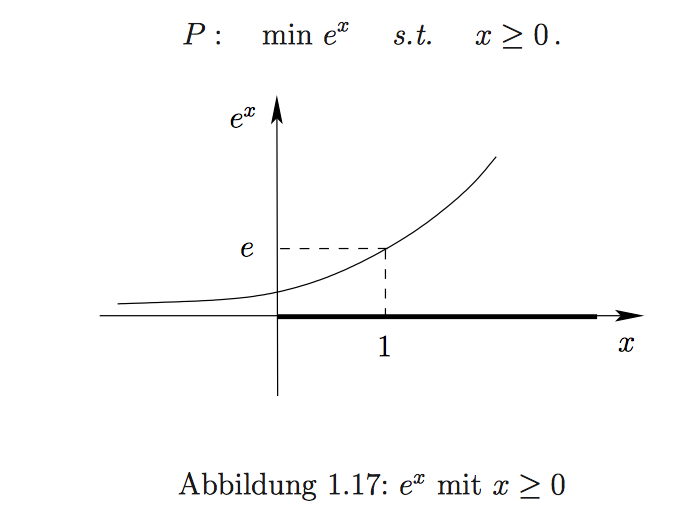
\includegraphics[scale=0.5]{img/ks-i}
	\end{figure*}
	~\\
	Hier ist $M = \big\{ x \in \R ~|~x \geq 0 \big\}$ unbeschränkt, der Satz von Weierstraß (Satz 1.2.10) also nicht anwendbar. Aber beispielsweise mit $\alpha = e$ ist
	$$ \operatorname{lev}_{\leq}^{e}(f, M) = \big\{ x \in M ~|~e^x \leq e \big\} = \big\{ x \geq 0 ~|~x \leq 1 \big\} = [0, 1] $$
	nicht-leer und kompakt. Folglich ist der Verschärften Satz von Weierstraß (Satz 1.2.16) anwendbar und $P$ daher lösbar.
\end{beispiel}

\begin{korollar}[1.2.19, Verschärfter Satz von Weierstraß für unrestringierte Probleme]
Sei $f \colon \R^n \rightarrow \R$ stetig und mit einem $\alpha \in \R$ sei $f_{\leq}^{\alpha}$ nicht-leer und kompakt. Dann ist auch $S$ nicht-leer und kompakt.	
\end{korollar}

\begin{definition}[1.2.23, Koerzivität bei $\infty$]
	Gegeben sei eine Funktion $f \colon M \rightarrow \R$ mit $M \subseteq \R^n$. Falls für alle Folgen $(x^\nu) \subseteq M$ mit $\lim_\nu \| x^\nu \| \rightarrow +\infty$ auch
	$$ \lim_\nu f(x^\nu) = +\infty $$
	gilt, dann heißt $f$ koerziv bei $\infty$ auf $M$. Falls $M$ abgeschlossen ist, heißt $f$ kurz koerziv auf $M$.
\end{definition}

\begin{beispiel}[1.2.28, Beispiel]
	Auf kompakten Mengen $M$ ist jede Funktion $f$ trivialerweise koerziv.
\end{beispiel}
 
\begin{lemma}[1.2.29]
	Die Funktion $f \colon M \rightarrow \R$ sei koerziv bei $\infty$ auf der Menge $M \subseteq \R^n$. Dann sind die Mengen $\operatorname{lev}_{\leq}^{\alpha}(f, M)$ für jedes Niveau $\alpha \in \R$ beschränkt.	
\end{lemma}

\begin{korollar}[1.2.30]
	Es sei $M$ nicht-leer und abgeschlossen und $f \colon M \rightarrow \R$ sei stetig und koerziv auf $M$. Dann ist $S$ nicht-leer und kompakt.
\end{korollar}

\begin{bemerkung}[1.2.35]
	Auf der abgeschlossenen Menge $X \subseteq \R^n$ seien die Funktionen $f, g_i$, $i \in I$, stetig, die Menge 
	$$ \big\{ x \in X ~|~g_i(x) \leq0, i \in I \big\} $$
	 sei nicht-leer, und mindestens eine der Funktionen $f, g_i$, $i \in I$, sei koerziv auf $X$. Zeigen Sie, dass die Menge $S$ der Optimalpunkte von $f$ auf $M$ dann nicht-leer und kompakt ist.
\end{bemerkung}


\begin{definition}[1.2.37, Koerzivität]
	Gegeben seien eine (nicht notwendigerweise abgeschlossene) Menge $M \subseteq \R^n$ und eine Funktion $f \colon M \rightarrow \R$. Falls für alle Folgen $(x^\nu) \subseteq M$ mit $\lim_\nu \| x^\nu \| \rightarrow \infty$ und alle konvergenten Folgen $(x^\nu) \subseteq M$ mit $\lim_\nu x^\nu \notin M$ die Bedingung 
	$$ \lim_\nu f(x^\nu) = +\infty $$
	gilt, dann heißt $f$ \textbf{koerziv} auf $M$.
\end{definition}

\begin{beispiel}[1.2.36, 1.2.38]
	Gegeben seien $N$ Beobachtungen $\hat{x}_1, \dotsc, \hat{x}_N \geq 0$ mit $\overline{x} = \frac{1}{N} \sum_{i=1}^{N} \hat{x}_i > 0$, die als Realisierungen stochastisch unabhängiger und mit Parameter $\lambda > 0$ exponentialverteilerter Zufallsvariablen $X_1, \dotsc, X_N$ aufgefasst werden. Gesucht ist der Parameter $\lambda$, der zu den Beobachtungen \enquote{am besten passt}. Dazu kann man mit Hilfe der Dichtefunktionen der einzelnen $X_i$,
	$$ f(\lambda x_i) = \begin{cases}
		\lambda e^{-\lambda x_i}, & x_i \geq 0 \\ 0, & x_i < 0,
	\end{cases} $$
	zunächst die gemeinsame Dichte aller Zufallsvariabelen
	$$ L(\lambda, x) = \Pi_{i=1}^{N} f(\lambda, x_i) $$
	betrachten. Der Maximum-Likelihood-Schätzer bestimmt dann $\lambda$ als optimalen Punkt des Problems
	$$ ML: \quad \max_{\lambda} L(\lambda, \tilde{x}) \text{ s.t. } \lambda > 0. $$
	Die zulässige Menge $M = (0, \infty)$ dieses Problems ist offensichtlich nicht abgeschlossen. Es sit auch sinnlos, den Parameterwert $\lambda = 0$ künstlich hinzuzufügen, da $f(0, x)$ keine Wahrscheinlichkeitsdichte ist. ~\\
	
	Wir werden im Folgendens sehen, wie die Lösbarkeit dieses Problems trotzdem garantiert werden und später auch einen globalen Maximalpunkt bestimmen. Dazu berechnen wir zunächst
	$$ L(\lambda, \hat{x}) = \Pi_{i=1}^{N} \lambda e^{-\lambda \hat{x}_i} = \lambda^N e^{-\lambda N \overline{x}}, \ell(\lambda, \hat{x}) \coloneqq \log(L(\lambda, \hat{x})) = N \log(\lambda) - \lambda N \overline{x} $$
	Da die Funktion $\log$ streng monoton wachsend auf dem Bildbereich $(0, \infty)$ von $L$ ist, kann man Hilfe von Übung 1.3.5 zeigen, dass das Problem
	$$ ML_{log}: \quad \max_\lambda \ell(\lambda, \hat{x}) \text{ s.t. } \lambda > 0 $$
	dieselben Optimalpunkte wie $ML$ besitzt. Schließlich streichen wir mittels Übung 1.3.1a) die Konstante $N > 0$ aus der Zeilfunktion und gehen zum äquivalenten Minimierungsproblem
	$$ P_{LM}: \quad \min_\lambda \lambda \overline{x} - \log(\lambda) \text{ s.t. } \lambda > 0 $$
	über.
	
% todo  kann man Hilfe von Übung 1.3.5 zeigen, dass das Problem ... Schließlich streichen wir mittels Übung 1.3.1a) die Konstante N

	Für $\overline{x} > =$ ist die Zielfunktion $f(\lambda) = \lambda \overline{x} - \log(\lambda)$ des Problems $P_{ML}$ koerziv auf $M = (0, \infty)$. Wir merken an, dass nur die Log-Likelihood-Funktion $\ell$ zu Koerzivität führt, die Likelihood-Funktion $L$ selbst aber nicht. ~\\
	
	Das Problem $P_{ML}$ und damit auch das Problem $ML$ sind nach Korollar 1.2.40 lösbar.
\end{beispiel}

\begin{lemma}[1.2.39]
	Die Funktion $f \colon M \rightarrow \R$ sei stetig und koerziv auf der Menge $M \subseteq \R^n$. Dann sind die Mengen $\operatorname{lev}_{\leq}^{\alpha}(f, M)$ für jedes Niveau $\alpha \in \R$ kompakt.
\end{lemma}

\begin{korollar}[1.2.40]
	Es sei $M$ nicht-leer, und $f \colon M \rightarrow \R$ sei stetig und koerziv auf $M$. Dann ist $S$ nicht-leer und kompakt.
\end{korollar}
% todo 1.2.40 Wichtiger satz für existence
\begin{bemerkung}[Rechenregeln] ~\
	\begin{itemize}
		\item Skalare und Vielfache (1.3.1) $\alpha \geq 0: ~ \min_{x \in M} \left( \alpha f(x) + \beta \right) = \alpha \left( \min_{x \in M} f(x) \right) + \beta$,
			$$ \alpha < 0:  \min_{x \in M} \left( \alpha f(x) + \beta \right) = \alpha \left( \max_{x \in M } f(x) \right) + \beta, \quad \min_{x \in M} \left( f(x) + g(x) \right) \geq \min_{x \in M} f(x) + \min_{x \in M} g(x) $$
		\item $\min_{x \in X} \max_{y \in Y} f(x, y) \geq \max_{y \in Y} \min_{x \in X} f(x, y)$
		 \item Monotone Transformation (1.35) $M \subseteq \R^n$, $f \colon M \rightarrow Y$ und $\psi \colon Y \rightarrow \R$ eine streng monotone wachsende Funktion. Dann gilt
		 	$$ \min_{x \in M} \psi(f(x)) = \psi (\min_{x \in M} f(x)) $$
		 \item Projektionsumformulierung (1.3.6): folgende Probleme sind äquivalent
		 	$$ P: \quad \min_{(x,y) \in \R^n \times \R^m} f(x) \text{ s.t. } (x, y) \in M $$
		 	und
		 	$$ P_{proj}: \quad \min_{x \in \R^n} f(x) \text{ s.t. } x \in \operatorname{pr}_x M $$
		 \item Monotones Funktional (1.3.8): wir nennen $F \colon \R^k \rightarrow \R$ monoton, falls $x \leq y \Rightarrow F(x) \leq F(y)$.
	\end{itemize}
\end{bemerkung}

\begin{bemerkung}[1.3.7, Epigraph Umformulierung]
	Gegeben seien $M \subseteq \R^n$ und eine Funktion $f \colon M \rightarrow \R$. Dann sind die folgenden Probleme äquivalent:
	$$ P: \quad \min_{x \in \R^n} f(x) \text{ s.t. } x \in M $$
	und 
		$$ P_{epi}: \quad \min_{(x, \alpha) \in \R^n \times \R} \alpha \text{ s.t. } f(x) \leq \alpha, x\in M $$
\end{bemerkung}

\begin{bemerkung}[1.3.9, Verallgemeinerte Epigraph Umformulierung]
	Gegeben seien $X \subseteq \R^n$, Funktionen $f \colon X \rightarrow \R^k$ und $g \colon X \rightarrow R^\ell$ sowie monotone Funtkionen $F \colon \R^k \rightarrow \R$ und $G \colon \R^\ell \rightarrow \R$. Dann sind die folgenden Probleme äquivalent:
	$$ P: \quad \min_{x \in \R^n} F(f(x)) \text{ s.t. }~ G(g(x)) \leq 0, x \in M $$
	und 
		$$ P_{epi}: \quad \min_{(x, \alpha, \beta) \in \R^n \times \R^k \times \R^\ell} F(\alpha) ~\text{ s.t. }~ G(\beta) \leq 0,  f(x) \leq \alpha, ~ g(x) \leq \beta, ~ x\in M $$
\end{bemerkung}

\chapter{Konvexe Optimierungsprobleme}

\section{Konvexität}

\begin{definition}[2.1.1, Konvexe Mengen und Funktionen] ~\
	\begin{enumerate}
		\item Eine Menge $M \subseteq \R^n$ heißt konvex, falls $\forall x, y \in M, \lambda \in (0, 1)$: $(1 - \lambda) x + \lambda y \in M$ gilt. Konvexe Mengen brauchen weder beschränkt noch abgeschlossen zu sein.
		\item Für eine konvexe Menge $M \subseteq \R^n$ heißt eine Funktion $f \colon M \rightarrow \R$ konvex, falls
			$$ \forall x, y \in M, \lambda \in (0, 1): \quad f( (1-\lambda)x + \lambda y) \leq (1- \lambda) f(x) + \lambda f(y) $$
			d.h. der Funktionsgraph von $f$ verläuft unter jeder seiner Sekanten.
		\item Für eine konvexe Menge $M \subseteq \R^n$ heißt eine Funktion $f \colon M \rightarrow \R$ strikt konvex, falls in b) für $x \ne y$ sogar die strikte Ungleichung gilt.
		\item Für eine konvexe Menge $M \subseteq \R^n$ heißt eine Funktion $f \colon M \rightarrow \R$ gleichmäßig konvex (auf $M$), falls mit einer Konstanten $c > 0$ die Funktion $f(x) - \frac{c}{2} \| x \|_2^2$ konvex auf $M$ ist.
		\item Für eine konvexe Menge $M \subseteq \R^n$ heißt eine Funktion $f \colon M \rightarrow \R$ konkav, strikt konkav oder gleichmäßig konkav (auf $M$) falls $-f$ konvex, strikt konvex bzw. gleichmäßig konvex auf $M$ ist.
	\end{enumerate}
\end{definition}

\begin{uebung}[2.1.2] % todo Uebung
	Auf einer konvexen Menge $M \subseteq \R^n$ ist die Funktion $f \colon M \rightarrow \R$ genau dann konvex, wenn die Mengen $\operatorname{epi}(f, M)$ konvex ist.	
\end{uebung}

\begin{definition}[2.1.3, Konvexes Optimierungsproblem]
	Das Optimierungsproblem
	$$ P: \quad \min f(x) \text{ s.t. } x \in M $$
	heißt \textbf{konvex}, falls $M$ und $f \colon M \rightarrow \R$ konvex sind. ~\\
	
	Da $M = \R^n$ eine konvexe Menge ist, sind unrestringierte Probleme genau dann konvex, wenn $f$ konvex auf $\R^n$ ist.
\end{definition}

\begin{satz}[2.1.4]
	$P$ sei konvex. Dann ist jeder lokale Minimalpunkt von $P$ auch globaler Minimalpunkt von $P$. ~\\
	
	Der Grund für diesen Effekt liegt darin, dass Konvexität eine globale Voraussetzung an $P$ ist.	
\end{satz}

\begin{uebung}[2.1.5] % todo Uebung
	Die Menge $M \subseteq \R^n$ und die Funktion $f \colon M \rightarrow \R$ seien konvex. Dann ist $\operatorname{lev}_{\leq}^{\alpha}(f, M)$ für jedes $\alpha \in \overline{\R}$ konvex. Die Umkehrung dieser Aussage ist falsch.	
\end{uebung}

\begin{uebung}[2.1.6]
	Der Schnitt beliebig vieler konvexer Mengen ist konvex.	
\end{uebung}

\begin{korollar}[2.1.8]
	Mit beliebigen Indexmengen $I, J$ seien die Funktionen $g_i \colon \R^n \rightarrow \R$, $i \in I$, konvex, und die Funktionen $h_j \colon \R^n \rightarrow \R$, $j \in J$, linear. Dann ist die Menge
	$$ M = \big\{ x \in \R^n ~|~g_i(x) \leq 0, i \in I, h_j(x) = 0, j \in J \big\} $$
	konvex.
\end{korollar}

\begin{beispiel}[2.1.9]
	Falls $f, g_i$ auf $\R^n$ konvex und $h_j$ lineare Funktionen sind, dann ist
	$$ P: \quad \min f(x) \text{ s.t. } g_i(x) \leq 0, ~ i \in I,~h_j(x) = 0, ~j \in J $$	
	ein konvexes Optimierungsproblem.
\end{beispiel}

\begin{beispiel}[2.1.10]
	Mit $c \in \R^n$, $b \in \R^m$ und einer $(m, n)$-Matrix $A = (a_1^T, \dotsc, a_m^T)^T$ mit $a_i \in \R^n$ ist
	$$ P: \quad \min c^T x \text{ s.t. } Ax \leq b $$
	ein lineares Optimierungsproblem (die Ungleichungsnebenbedingungen können sowohl eine Nichtnegativitätsbedingung $x \geq 0$ enthalten als auch Gleichungen modellieren). ~\\
	
	$P$ ist auch ein konvexes Optimierungsproblem, denn mit den Setzungen $f(x) = c^T x$, und $g_i(x) = a_i^T x - b_i$ sind $f, g_i \colon \R^n \rightarrow \R$ linear und damit konvex auf $\R^n$. ~\\
	
	Zum Beispiel setzt man für das lineare Optimierungsproblem
	$$ \min x_1 + x_2 \text{ s.t. } x \geq 0 $$
	$f(x) = x_1 + x_2$, $g_1(x) = - x_1$ und $g_2(x) = -x_2$.
\end{beispiel}

\newpage

\section{$C^1$-Charakterisierung}

\begin{bemerkung}[Kettenregel] $D(f \circ g)(\overline{x}) = D f(g(\overline{x})) \cdot D g(\overline{x})$	
\end{bemerkung}

\begin{satz}[2.2.1, Linearisierung per Satz von Taylor im $\R^n$]
	Für eine nicht-leere, offene und konvexe Menge $U \subseteq \R^n$ sei die Funktion $f \colon \rightarrow \R$ differenzierbar an $x \in U$. Dann gilt für alle $y \in U$	
	$$ f(y) = f(x) + \langle \nabla f(x), y - x \rangle + o \left( \| y - x \| \right), $$
	wobei $o \left( \| y - x \| \right)$ einen Ausdruck der Form $w(y) \| y - x \|$ mit einer an $x$ stetigen Funktion $w$ mit $w(x) = 0$ bezeichnet.
\end{satz}

\begin{satz}[2.2.2., $C^1$-Charakterisierung von Konvexität]
	Auf einer konvexen Mengen $M \subseteq \R^n$ ist eine Funktion $f \in C^1(M, \R)$	 genau dann konvex, wenn folgendes gilt
	$$ \forall x, y \in M: \quad f(y) \geq f(x) + \langle \nabla f(x), y - x \rangle $$
	Die $C^1$-Charakterisierung besagt, dass eine $C^1$-Funktion genau dann konvex auf $M$ ist, wenn ihr Graph über jeder seiner Tangentialebenen verläuft.
\end{satz}

\newpage

\section{Lösbarkeit}

Für die Lösbarkeit von $P$ ist Konvexität alleine kein wesentlicher Vorteil: sowohl $f_1(x) = (x - 5)^2$ als auch $f_2(x) = e^x$ sind sogar strikt konvex, aber nur $f_1$ besitzt einen globalen Minimalpunkt auf $\R$. Im Folgenden werden wir sehen, dass der entscheidende Vorteil von $f_1$ gegenüber $f_2$ die gleichmäßige Konvexität ist.

\begin{uebung}[2.3.1] % todo Uebung
	Für eine konvexe Menge $M \subseteq \R^nle$ sei $f \colon M \rightarrow \R$ gleichmäßig konvex. Dann ist $f$ auch strikt konvex auf $M$.	
\end{uebung}

\begin{lemma}[2.3.2]
	Für eine abgeschlossene und konvexe Menge $M \subseteq \R^n$ sei $f \colon M \rightarrow \R$ gleichmäßig konvex. Dann ist $f$ auch
	\begin{enumerate}
		\item koerziv auf $M$ und
		\item stetig auf dem Inneren von $M$.
	\end{enumerate}
\end{lemma}

% todo 2.3.3 Wichtiger Eindeutigkeit
\begin{satz}[2.3.3]
	$P$ sei konvex. Dann gelten die folgenden Aussage:
	\begin{enumerate}
		\item Die Menge der Minimalpunkte ist konvex.
		\item Falls $f$ strikt konvex auf $M$ ist, dann besitzt $S$ höchstens ein Element.
		\item Es sei $M$ nicht-leer und abgeschlossen, und $f$ sei gleichmäßig konvex und stetig auf $M$. Dann besitzt $S$ genau ein Element (d.h. $P$ ist eindeutig lösbar).
	\end{enumerate}	
	Angemerkt sei, dass die Stetigkeitsforderung an $f$ in Satz 2.3.3c) nach Lemma 2.3.2b) unnötig ist, falls die Menge $M$ mit ihrem Inneren übereinstimmt (z.B. für $M = \R^n$).
\end{satz}

\newpage

\section{Optimalitätsbedingungen für unrestringierte Probleme}

Wir betrachten im Folgenden das unrestringierte Problem 
$$ P: \quad \min f(x). $$
Allgemeiner bezeichnet man auch Probleme mit offener zulässiger Menge $M$ als unrestringiert. In der Tat lassen sich die im Folgenden besprochenen Optimalitätsbedingungen ohne weiteres auf diesen Fall übertragen, was wir aus Gründen der Übersichtlichkeit aber nicht explizit angeben werden.

\begin{definition}[2.4.1, Kritischer Punkt]
	Ein Punkt $\overline{x} \in \R^n$ heißt kritisch für $f \in C^1(\R^n, \R)$, falls $\nabla f(\overline{x}) = 0$ gilt.	
\end{definition}

\begin{satz}[2.4.2, Fermat'sche Regel, notwendige Optimalitätsbedingung]
	Der Punkt $\overline{x} \in \R^n$ sei lokal minimal für $f \in C^1(\R^n, \R)$. Dann ist $\overline{x}$ kritischer Punkt von $f$. Achtung dies ist lediglich notwendig und nicht hinreichend.
\end{satz}

\begin{beispiel}[2.4.3, Fortsetzung von 1.1.5 - Zentrum einer Punktewolke] ~\\
	Gegeben seien Punkte $x^1, x^2, \dotsc, x^m \in \R^n$. Gesucht ist ein Punkt $z \in \R^n$ \enquote{im Zentrum der Punkte}. Benutzt man die 2-Norm so führt dies auf das Optimierungsproblem
		$$ P: \quad \min_{z \in \R^n} \left\| \left( \| z - x^2 \|_2, \dotsc \| z - x^m \|_2 \right)^T \right\|_2, $$
	ohne Nebenbedingungen. Als Optimalpunkt berechnet man das arithmetische Mittel der Punkte
	$$ \overline{z} = \frac{1}{m} \sum_{i=1}^m x^i. $$
	Beweis hiervon folgt aus:
	$$ f(z) = \sqrt{ \sum_{i=1}^{m} \| z - x^i \|_2^2} = \sqrt{ m z^T z - 2 z^T \sum_{i=1}{m} x^i + \sum_{i=1}^{m} \| x^i \|_2^2} $$
	so dass $f$ nicht differenzierbar it und Satz 2.4.2 nicht angewendet werden kann. Nach Übung 1.3.5 mit $\psi(y) = y^2$ und $Y = \{ y \in \R ~|~y \geq 0  \}$ besitzt $f$ aber dieselben Minimalpunkte wie die stetig differenzierbare Funktion
	$$ f^2(z) = mz^Tz - 2z^T \sum_{i=1}^{m} x^i + \sum_{i=1}^{m} \| x^i \|_2^2 $$
	Kritische Punkte dieser Funktion sind genau die Lösungen der Gleichung 
	$$ 0 = \nabla \left( f^2(z) \right) = 2 mz - 2 \sum_{i=1}^m x^i $$
	also besitzt $f^2$ den eindeutigen kritischen Punkt
	$$ \overline{z} = \frac{1}{m} \sum_{i=1}^{m} x^i $$
	Tatsächlich ist $\overline{z}$ auch globaler Minimalpunkt von $F^2$ sowie von $f$, wie man durch folgende Argumente sieht: nach Beispiel 1.2.31 existiert zunächst ein globaler Minimalpunkt $\tilde{z}$ von $f$ und damit auch von $f^2$ auf $\R^n$. Aufgrund der Fermat'schen Regel (Satz 2.4.2) muss $\tilde{z}$ kritischer Punkt von $f^2$ ist aber das gerade berechnete $\overline{z}$, so dass nur $\tilde{z} = \overline{z}$ gelten kann. Also ist $\overline{z}$ globaler Minimalpunkt von $f$ auf $\R^n$. ~\\
	
	In Kapitel 2.5 werden wir außerdem nachweisen, dass $f^2$ eine auf $\R^n$ konvexe Funktion ist, was es ermöglichen wird, die globale Minimalität von $\overline{z}$ alternativ zu beweisen, ohne zunächst die Lösbarkeit des zugrundeliegenden Optimierungsproblems zu zeigen.
\end{beispiel}

\begin{beispiel}[2.4.4, Fortsetzung von 1.2.36]
	Die Zielfunktion $f(\lambda) = \lambda \overline{x} - \log(\lambda)$ mit $\overline{x} > 0$ des Problems $P_{ML}$ aus Beispiel 1.2.36	erfüllt $f'(\lambda) = \overline{x} - \frac{1}{\lambda}$, besitzt als eindeutiges kritischen Punkt also $\overline{\lambda} = \frac{1}{\overline{x}}$. ~\\
	
	Wie in Beispiel 2.4.3 lässt sich nun argumentieren, dass $\overline{\lambda} = \frac{1}{\overline{x}}$ globaler Minimalpunkt von $P_{ML}$ und damit der gesuchte Maximum-Likelihood-Schätzer der Exponentialverteilung ist: nach Beispiel 1.2.41 existiert zunächst ein globaler Minimalpunkt $\tilde{\lambda}$ von $P_{ML}$. Da sich Optimierungsprobleme mit offenen zulässigen Mengen wie unrestringierte Optimierungsprobleme behandeln lassen, muss $\tilde{\lambda}$ nach der Fermat'schen Regel ein kritischer Punkt von $f$ sein. Einzig kritischer Punkt von $f$ ist aber das gerade berechnete $\tilde{\lambda}$, woraus die Behauptung folgt. ~\\
	
	In Kapitel 2.5 werden wir außerdem sehen, dass $f$ auf der zulässigen Menge $(0, \infty)$ von $P_{ML}$ konex ist, was es wieder ermöglichen wird, die globale Minimaliität von $\overline{\lambda}$ alternativ zu beweisen, ohne zunächst die Lösbarkeit von $P_{ML}$ zu zeigen.
\end{beispiel}


\begin{satz}[2.4.5, Hinreichende Optimalitätsbedingung]
	$f \in C^1(\R^n, \R)$ sei konvex. Dann ist jeder kritische Punkt von $f$ globaler Minimalpunkt von $f$.
\end{satz}

\begin{korollar}[2.4.6, Charakterisierung globaler Minimalpunkte]
	$f \in C^1(\R^n, \R)$ sei konvex	 Dann sind die globalen Minimalpunkte genau die kritischen Punkte von $f$.
\end{korollar}

Zur Bestimmung globaler Minimalpunkte unrestringierter konvexer $C^1$-Probleme genügt es also nicht nur, lokale Minimalpunkte zu suchen (wie schon in Satz 2.1.4 gesehen), sondern sogar nur kritische Punkte. Das globale Minimierungsproblem ist damit auf das Lösen der Gleichung $\nabla f(x) = 0$ zurückgeführt. ~\\

Insbesondere erhält man auch diese Aussage: falls $f$ keinen kritischen Punkt besitzt, dann auch keinen globalen Minimalpunkt. Dazu muss allerdings bewiesen werden, dass $f$ keinen kritischen Punkt besitzen kann (ein einfaches Beispiel hierfür ist $f(x) = e^x$).

\newpage

\section{$C^2$-Charakterisierung von Konvexität}

\begin{satz}[2.5.1, Quadratische Approximation per Satz von Taylor im $\R^n$]
	Für eine nicht-leere, offene und konvexe Menge $U \subseteq \R^n$ sei die Funktion $f \colon U \rightarrow \R$ zweimal differenzierbar an $x \in U$. Dann gilt für alle $y \in U$
	$$ f(y) = f(x) + \langle \nabla f(x), y - x \rangle + \frac{1}{2} \left( y - x \right)^T D^2 f(x) (y - x) + o\left( \| y - x \|^2 \right) $$	
	Der Fehlerterm lässt sich dabei auch mit Hilfe des Lagrange-Restgliedes angeben:
	$$ o\left( y - x \|^2 \right) = \frac{1}{2} \left( y - x \right)^T D^2 f(\xi) (y - x ) - \frac{1}{2} \left(y - x \right)^T D^2 f(x) (y -x ), $$
	wobei $\xi$ ein nicht näher bekannter Punkt auf der Verbindungsstrecke zwischen $x$ und $y$ ist.
\end{satz}

\begin{definition}
	Eine symmetrische $(n, n)$-Matrix $A$ heißt \textbf{positiv semidefinit} (kurz: $A \succeq 0$), wenn
	$$ \forall x \in \R^n: \quad x^T A x \geq 0 $$
	gilt, und \textbf{positiv definit} (kurz: $A \succ 0$), wenn die Ungleichung für alle $x \neq 0$ sogar strikt ist. ~\\
	
	In der Linearen Algebra wird allerdings gezeigt, dass $A \succeq 0$ ($\succ 0$) genau dann gilt, wenn $\lambda \geq 0$ ($> 0$) für alle Eigenwerte $\lambda$ von $A$ gilt. 
\end{definition}

\begin{satz}[2.5.2, Notwendige Optimalitätsbedingung zweiter Ordnung]
	Der Punkt $\overline{x}$ sei lokaler Minimalpunkt von $f \colon \R^n \rightarrow \R$, und $f$ sei an $\overline{x}$ zweimal differenzierbar. Dann gilt $\nabla f(\overline{x}) = 0$ und $D^2 f(\overline{x}) \succeq 0$.
\end{satz}

\subsection*{$C^2$-Charakterisierung von Konvexität}

\begin{satz}[2.5.3, $C^2$-Charakterisierung von Konvexität]
	Auf einer konvexen Menge $M \subseteq \R^n$ sei die Funktion $f \in C^2(M, \R)$	gegeben. 
	\begin{enumerate}
		\item Falls $\forall x \in M$: $D^2 f(x) \succeq 0$ gilt, dann ist $f$ auf $M$ konvex.
		\item Falls $M$ außerdem offen ist, dann gilt auch die Umkehrung der Aussage in Teil a).
	\end{enumerate}
	Dass die Voraussetzung der Offenheit von $M$ in b) nicht nur beweistechnischer Natur ist, sieht man an der $C^2$-Funktion $f(x) = x_1^2 - x_2^2$, die nirgends eine positiv semidefinite Hessematrix besitzt, aber trotzdem auf der Menge $M = \R \times \{ 0 \}$ konvex ist. $M$ ist in diesem Beispiel natürlich nicht offen. ~\\
	
	Die Voraussetzung der Offenheit von $M$ in Satz 2.5.3b) lässt sich zur Volldimensionalität von $M$ abschwächen, also im Wesentlichen zur Forderung, dass $M$ innere Punkte besitzt. Eine weitergehende Abschwächung ist nicht möglich.
\end{satz}

\begin{beispiel}[2.5.3]
	Die Funktion $f(x) = (x - 5)^2$ erfüllt $f''(x) = 2 \geq 0$ für alle $x \in \R$ und ist damit konvex auf $\R$.	
\end{beispiel}

\begin{beispiel}[2.5.5]
	Die Funktion $f(x) = e^x$ erfüllt $f''(x) = e^x \geq 0$ für alle $x \in \R$ und ist damit konvex auf $\R$.	
\end{beispiel}

\begin{beispiel}[2.5.6, Fortsetzung von 1.1.5]
	Für den Gradienten der Funktion $f^2$ auf Beispiel 2.4.3 haben wir bereits die Darstellung 
	$$ \nabla \left( f^2(z) \right) = 2 mz - 2 \sum_{i=1}^{m} x^i $$	
	hergeleitet, woraus
	$$ D^2 \left( f^2(z) \right) = 2mE \text{ (mit der $(n,n)$-Einheitsmatrix $E$)} $$
	folgt. Damit besitzt $D^2 f^2(z)$ den $n$-fachen Eigenwert $2m \geq 0$. Hieraus folgt die Konvexität von $f^2$ auf $\R^n$. ~\\
	
	Nach Korollar 2.4.6 ist jeder kritische Punkt von $f^2$ globaler Minimalpunkt von $f^2$ und damit auch von $f$, und der (einzige) kritische Punkt von $f^2$ ist das in Beispiel 2.4.3 berechnete arithmetische Mittel $\overline{z}$ der Punktewolke. Damit ist alternativ zur Argumentation in Beispiel 2.4.3 die globale Minimalität von $\overline{z}$ gezeigt, ohne zuvor die Lösbarkeit des Optimierungsproblems nachzuweisen.
\end{beispiel}

\begin{beispiel}[2.5.7, Fortsetzung von 1.2.36]
	Die Funktion $f(\lambda) = \lambda \overline{x} - \log(\lambda)$ mit $\overline{x} > 0$ auf Beispiel 2.4.4 erfüllt $f'(\lambda) = \overline{x} - \frac{1}{\lambda}$ und $f''(\lambda) = \frac{1}{\lambda^2} \geq 0$ für alle $\lambda \in (0, \infty)$. Sie ist damit konvex auf $(0, \infty)$. Die Konvex von $f$ korrespondiert zur Konkavität der Log-Likelihood-Funktion $\ell$. Wir bemerken, dass die Likelihood-Funktion $L$ selbst nicht konkav ist. ~\\
	
	Der in Beispiel 2.4.4 berechnete kritische Punkt $\overline{\lambda} = \frac{1}{\overline{x}}$ von $f$ ist nach Korollar 2.4.6 wieder globaler Minimalpunkt von $P_{ML}$ und damit der gesuchte Maximum-Likelihood-Schätzer der Exponentialverteilung. Auch bei diesem Argument sit (alternativ zu dem in Beispiel 2.4.4) die Betrachtung der Lösbarkeit von $P_{ML}$ unnötig.
\end{beispiel}

\begin{uebung}[2.5.8, Fortsetzung von Beispiel 1.1.6]
	Die Zielfunktion 
	$$ f(z^1, \dotsc, z^k) = \sum_{i=1}^{m} \min_{\ell=1, \dotsc, k} \| z^\ell - x^i \| = \left\| \left( \| z^{\ell(1)} - x^1 \|, \dotsc, \| z^\ell(m) - x^m \| \right)^T \right\|_1 $$	
	mit $k \geq 2$ aus dem Problem $P_1$ der Clusteranalyse (Bsp. 1.1.6) ist nicht konvex auf $\R^{nk}$ (wenn die Indizes $\ell(i)$, $i =1, \dotsc, m$, allerdings a priori bekannt sind, dann lässt mit einem anderen Argument als der Benutzung von Satz 2.5.3 zeigen, dass $f$ doch konvex ist).
\end{uebung}

\begin{uebung}[2.5.9, Hinreichende Bedingung für strikte Konvexität]
	Auf einer konvexen Menge $M \subseteq \R^n$ sei die Funktion $f \in C^2(M, \R)$ gegeben, und es gelte
	$$ \forall x\in M: \quad D^2 f(x) \succ 0 $$
	Dann ist $f$ auf $M$ strikt konvex.	
\end{uebung}

\begin{satz}[2.5.10, $C^2$-Charakterisierung von gleichmäßiger Konvexität]
	Auf einer konvexen Menge $M \subseteq \R^n$ sei die Funktion $f \in C^2(M, \R)$ gegeben.
	\begin{enumerate}
		\item Falls mit einer Konstanten $c > 0$
		$$ \forall x \in M: \quad \lambda_{min} \left( D^2 f(x) \right) \geq c $$
		gilt, dann ist $f$ auf $M$ gleichmäßig konvex.
		\item Falls $M$ außerdem offen ist, dann gilt auch die Umkehrung der Aussage in Teil a)
	\end{enumerate}	
\end{satz}

\begin{beispiel}[2.5.11]
	Die Funktion $f(x) = (x - 5)^2 $ erfüllt $f''(x) = 2 > 0$ für alle $x \in \R$ und ist damit nicht nur strikt, sondern sogar gleichmäßig konvex auf $\R$.	
\end{beispiel}

\begin{beispiel}[2.5.12]
Die Funktion $f(x) = e^x$ erfüllt $f''(x) = e^x > 0$ für alle $x \in \R$ und ist damit strikt konvex auf $\R$. Allerdings gilt $\lim_{x \rightarrow -\infty} f''(x) = 0$, so dass sie nicht gleichmäßig konvex auf $\R$ ist
\end{beispiel}

\begin{beispiel}[2.5.13, Fortsetzung von 1.1.5]
	Für die Hessematrix des Quadrats der Funktion $f$ aus Beispiel 1.1.5 haben wir in Beispiel 2.5.6 die Darstellung $D^2 f^2(z) = 2mE$ und damit den $n$-fachen Eigenwert $2m$ für jedes $z \in \R^n$ hergeleitet. Insbesondere gilt dann $\lambda_{min}(D^2 f^2(z)) = 2m > 0$ für alle $z \in \R^n$, woraus die strikte und sogar gleichmäßige Konvexität von $f^2$ auf $\R^n$ folgt. 
\end{beispiel}

\begin{beispiel}[2.5.14, Fortsetzung von 1.2.36]
	Die Funktion $f(\lambda) = \lambda \overline{x} - \log(\lambda)$ mit $\lambda{x} > 0$ aus Beispiel 1.2.36 erfüllt $f''(\lambda) = \frac{1}{\lambda^2} > 0$ für alle $\lambda \in (0, \infty)$, abere $\lim_{\lambda \rightarrow \infty} f''(\lambda) = 0$. Sie ist damit zwar strikt, aber nicht gleichmäßig konvex auf $(0, \infty)$. ~\\
	
	Nach Beispiel 1.2.38 ist $f$ trotzdem koerziv. Dies zeigt, dass die Bedingung für Koerzivität aus Lemma 2.3.2 nur hinreichend, aber nicht notwendig ist.
\end{beispiel}

\subsection*{Konvexität und Monotonie der ersten Ableitung}

Für $n = 1$, ein offenes Intervall $M \subseteq \R$ und eine Funktion $g \in C^1(M, \R)$ ist aus der Analysis bekannt, dass $g$ genau dann monoton wachsend auf $M$ ist, wenn $g'(x) \geq 0$ für alle $x \in M$ gilt. Nach Satz 2.5.3 gilt für $n = 1$, ein offenes Intervall $M \subseteq \R$ und $f \in C^2(M, \R)$ also, dass $f$ genau dann konvex auf $M$ ist, wenn $f'$ auf $M$ monoton wächst.  In $n = 1$ ist die Monotonie von $g$ äquivalent zur Gültigkeit der Ungleichung $(g(y) - g(x))(y - x) \geq 0$.. Die motiviert für das Mehrdimensionale die folgende Definition.

\begin{definition}[2.5.15, Monotoner Operator]
	Für eine nicht-leere konvexe Menge $M \subseteq \R^n$ heißt $g \colon M \rightarrow \R^n$ \textbf{monoton} auf $M$, falls folgendes gilt:
	$$ \forall x,y \in M: \quad \langle g(y) - g(x), y - x \rangle \geq 0 $$
\end{definition}

\begin{satz}[2.5.16, Monotonie-Charakterisierung von Konvexität]
	Auf einer konvexen Menge $M \subseteq \R^n$ ist eine Funktion $f \in C^1(M, \R)$ genau dann konvex, wenn $\nabla f$ auf $M$ monoton ist.	
\end{satz}

\newpage

\section{Dualität}

Wir betrachten das restringierte Optimierungsproblem 
	$$ P: \quad \min f(x) \text{ s.t. } g_i(x) \leq 0, i \in I, ~h_j(x) = 0, j \in J $$
mit $f, g_i, h_j \colon \R^n \rightarrow \R$, $I = \{ 1, \dotsc, p \}$, $J = \{ 1, \dotsc, q \}$, $p, q \in \N_0$ und $q < n$ (wobei z.B. $p = 0$ dem Fall $I = \emptyset$ entspricht, also der Abwesenheit von Ungleichungsrestriktionen). Zunächst setzen wir weder Konvexität noch Differenzierbarkeit der beteiligten Funktionen voraus.

\begin{definition}[2.6.1, Lagrang-Funktion]
	Die Funktion 
	$$ L(x, \lambda, \mu) = f(x) + \sum_{i \in I} \lambda_i g_i(x) + \sum_{j \in J} \mu_j h_j(x) $$
	mit $\mu = (\mu_1, \dotsc, \mu_p)^T$ und $\mu = ( \mu_1, \dotsc, \mu_p)^T$ heißt \textbf{Lagrangefunktion} von $P$. 
\end{definition}

Es sei zunächst $p = 0$. Dann gilt $L(x, \mu) = f(x) + \sum_{j \in J} \mu_j h_j(x)$ und 
	$$ \varphi(x) \coloneqq \sup_{\mu \in \R^q} L(x, \mu) = \begin{cases} f(x), & \forall j \in J: h_j(x) \text{ (d.h. falls } x \in M) \\ \infty, & x \notin M \end{cases} $$

\begin{beispiel}
	$J = \{ 1 \}$, $h_1(x) = x^2 - 1$, $f(x) = x$ führt zu der in Abbildung 2.9 skizzierten Funktion $\varphi$. Statt $P$ zu lösen kann man also formal auch die unrestringierte Funktion $\varphi(x)$ minimieren (\enquote{formal}, weil $\varphi$ nicht nach $\R$ abbildet, sondern nach $\overline{\R}$). Insbesondere gilt
	$$ v = \inf_{x \in M} f(x) = \inf_{x \in \R^n} \varphi(x) = \inf_{x \in \R^n} \sup_{\mu \in \R^q} L(x, \mu) $$	
\end{beispiel}

Nun sei $q = 0$. Dann gilt $L(x, \mu) = f(x) + \sum_{i \in I} \lambda_i g_i(x)$,
	$$ \varphi(x) \coloneqq \sup_{\lambda \geq 0} L(x, \lambda) = \begin{cases} f(x), & x \in M, \\ \infty, & x \notin M \end{cases} $$
und 
	$$ v = \inf_{x \in M} f(x) = \inf_{x \in \R^n} \varphi(x) = \inf_{x \in \R^n} \sup_{\lambda \geq 0} L(x, \lambda) $$

\begin{beispiel}
	$I = \{ 1 \}$, $g_(x) = x^2 - 1$, $f(x) = x$ führt zu der in Abbildung 2.10 skizzieren Funktion $\varphi$. Analog erhält man für beliebige $p, q \in \N_0$
		$$ \varphi(x) \coloneqq \sup_{\lambda \geq 0, \mu \in \R^q} L(x, \lambda, \mu) = \begin{cases} f(x), & x \in M \\ \infty, & x \notin M \end{cases} $$	
	und 
		$$ v = \inf_{x \in M} f(x) = \inf_{x \in \R^n} \varphi(x) = \inf_{x \in \R^n} \sup_{\lambda \geq 0, \mu \in \R^q} L(x, \lambda, \mu). $$
\end{beispiel}

Die zentrale Frage der Dualitätstheorie lautet, ob man in obiger Formel \enquote{$\inf$} und \enquote{$\sup$} vertauschen darf, ob also auch die folgende Formel gilt
	$$ v = \inf_{x \in M} f(x) = \sup_{\lambda \geq 0, \mu \in \R^q} \inf_{x \in \R^n} L(x, \lambda, \mu). $$
	
Das folgende Beispiel zeigt, dass diese Vertauschung nicht immer möglich ist.
	
\begin{beispiel}[2.6.2]
	Für $n = 1$, $p = 1$, $q = 0$, $f(x) = x^2$ und $g(x) = 1 - x^4 \leq 0$ berechnet man leicht $v = 1$. Andererseits gilt
		$$ L(x, \lambda) = x^2 + \lambda (1 - x^4) $$
	und damit 
		$$ \inf_{x \in \R} L(x, \lambda) = \begin{cases} - \infty, & \lambda > 0, \\ 0, & \lambda = 0 \end{cases} $$
	sowie
		$$ \sup_{\lambda \geq 0} \inf_{x \in \R} L(x, \lambda) = 0 < 1 = v $$
\end{beispiel}

Die Dualitätstheorie gibt Bedingungen an, unter denen solche Beispiele ausgeschlossen, sind, unter denen also Gleichheit gilt. Dazu fassen wir den Ausdruck 
	$$ \sup_{\lambda \geq 0, \mu \in \R^q} \inf_{x \in \R^n} L(x,\lambda, \mu) $$
	als Maximalwert eines Optimierungsproblem aus:
	$$ D: \quad \max_{\lambda, \mu} \psi(\lambda, \mu) \text{ s.t. } \lambda \geq 0 $$
	mit $\psi(\lambda, \mu) \coloneqq \inf_{x \in \R^n} L(x, \lambda, \mu)$.	
	
\begin{definition}[2.6.3, Lagrange-Dual]
	Das Problem $D$ heißt \textbf{Lagrange-Dual} von $P$. Seinen Maximalwert bezeichnen wir mit
	$$ v_D \coloneqq \sup_{\lambda \geq 0, \mu \in \R^q} \psi(\lambda, \mu) $$
	und seine zulässige Menge mit
	$$ M_D \coloneqq \{ (\lambda, \mu) \in \R^p \times \R^q ~|~\lambda \geq 0 \} $$
	Analog bezeichnen wir $P$ als primales Problem mit Minimalwert $v_P \coloneqq v$ und zulässiger Menge $M_P \coloneqq M$.
\end{definition}	

Die zentrale Frage der Dualitätstheorie lautet in dieser Notation, wann die Gleichheit
	$$ v_D = v_P $$
erfüllt ist.

\begin{satz}[2.6.4, Schwacher Dualitätssatz]
	Es gilt $v_D \leq v_P$.	
\end{satz}
	
Der Wert $v_P - v_D$ heißt Dualitätslücke. In Beispiel 2.6.2 beträgt die Dualitätslücke $v_P - v_D = 1$. In dieser Terminologie lautet die zentrale Frage der Dualitätstheorie, wann die Dualitätslücke verschwindet.	 ~\\

Die übliche Umformulierung dieser unendlich vielen Ungleichungen per Supremums- bzw. Infimumsbildung führt zu
	$$ \underbrace{\sup_{\overline{\lambda} \geq 0, \overline{\mu} \in \R^q} \inf_{x \in \R^n} L(x, \overline{\lambda}, \overline{\mu})}_{v_D} \leq \underbrace{\inf_{\overline{x} \in \R^n} \sup_{\lambda \geq 0, \mu \in \R^q} L(\overline{x}, \lambda, \mu)}_{v_P} $$
	
Im Folgenden sei $P$ ein konvexes Optimierungsproblem mit $f, g_i \in C^1(\R^n, \R)$, $i \in I$, und $h_j$, $j \in J$, linear. Kurz gesagt sei $P$ ab jetzt konvex und $C^1$. Dann ist die Lagrangefunktion
	$$ L(x, \lambda, \mu) = f(x) + \sum_{i \in I} \lambda_i g_i(x) + \sum_{j \in J} \mu_j h_j(x) $$
für beliebige fest vorgegebene $\lambda \geq 0$ und $\mu \in \R^q$ konvex und $C^1$ in der Variable $x$! \smallskip

Folglich ist für alle $\lambda \geq 0$, $\mu \in \R^n$ der Wert $\psi(\lambda, \mu) = \inf_{x \in \R^n} L(x, \lambda, \mu)$ der Minimalwert eines unrestringierten konvexen $C^1$-Problems. Falls dieses Infimum für alle $\lambda \geq 0$, $\mu \in \R^n$ als Minimalwert angenommen wird, lässt es sich mit Korollar 2.4.6 berechnen als
	$$ \psi(\lambda, \mu) = L(x^*, \lambda, \mu), $$
wobei $x^*$ einen globalen Minimalpunkt von $L(\cdot, \lambda, \mu)$ auf $\R^n$ bezeichnet, also eine Lösung $x^*$ von
$$ \nabla_x L(x, \lambda, \mu) = 0. $$

Das Dualproblem lässt sich dadurch folgendermaßen umformulieren:
	$$ D: \quad \max_{x, \lambda, \mu} L(x, \lambda, \mu) \text{ s.t. } \nabla_x L(x, \lambda, \mu) =0, ~ \lambda \geq 0 $$
(das sogenannte \textbf{Wolfe-Dual} von $P$), was im Gegensatz zum Lagrange-Dual ein numerisch gut handhabbares Problem ist.	Seine zulässige Menge wird nun zu
	$$ M_D = \{ (x, \lambda, \mu) \in \R^n \times \R^p \times \R^q ~|~\nabla_x L(x, \lambda, \mu) = 0, \lambda \geq 0 \}. $$
Einen Punkt $x \in M_P = M$ nennen wir im Folgenden \textbf{primal zulässig}, und $(x, \lambda, \mu) \in M_D$ \textbf{dual zulässig}. Schwache Dualität bedeutet jetzt
	$$ \sup_{(x, \lambda, \mu) \in M_D} L(x, \lambda, \mu) \leq \inf_{x \in M_P} f(x) $$
	Aufgrund der formalen Definitionen für Suprema und Infima über leere Mengen ist diese Ungleichung bemerkenswerterweise sogar für $M_D = \emptyset$ und/oder $M_P = \emptyset$ sinnvoll.
	
\begin{satz}[2.6.5] ~\
	\begin{enumerate}
		\item $\overline{x}$ sei primal zulässig. Dann ist $f(\overline{x})$ eine Oberschranke für den globalen Minimalwert von $P$:
			$$ v_P \leq f(\overline{x}) $$
		\item $(\overline{x}, \overline{\lambda}, \overline{\mu})$ sei dual zulässig. Dann ist $L(\overline{x}, \overline{\lambda}, \overline{\mu})$ eine Unterschrank für $v_P$:
			$$ v_P \geq L(\overline{x}, \overline{\lambda}, \overline{\mu}) $$
	\end{enumerate}	
\end{satz}
	
\begin{beispiel}[2.6.6, Abstand von einer Hyperebene]
	Gesucht ist der Abstand von $z \in \R^n$ zu swe Hyperebene $H = \{ x \in \R^n ~|~ a^Tx = b \}$	 mit $a \in \R^n \setminus \{ 0 \}$ und $b \in \R$. Im Folgende werden wir sehen, welche Aussagen die Dualitätstheorie für das allgemeine Problem
	$$ P: \quad \min_{x \in \R^n} \| x - z \|_2 \text{ s.t. } a^T x = b $$
	zulässt und diese an obigem speziellen Beispiel mit $a = (1, 2)$, $b = 2$ und $z = 0$
	$$ \min_{x \in \R^2} \| x\|_2 \text{ s.t. } x_1 + 2x_2 = 2 $$
	verdeutlichen. $P$ ist durch Quadrieren der Zielfunktion nach Übung 1.3.5 äquivalent zu
	$$ Q: \quad \min (x - z)^T(x - z) \text{ s. t. } a^T x = b $$
	In $Q$ ist die Zielfunktion $f(x) \coloneqq x^T x - 2z^T x + z^T z$ offenbar konvex und $C^1$, und die Gleichungsrestriktion $h(x) = a^Tx - b$ ist linear. Also ist $Q$ konvex und $C^1$ und damit für Dualitätsaussagen geeignet.
\end{beispiel}

\begin{lemma}[2.6.7]
	$P$ sei konvex und $C^1$, und es seien $\overline{x} \in \R^n$, $\overline{\lambda} \in \R^p$, $\overline{\mu} \in \R^q$ gegeben mit
	\begin{enumerate}
		\item $\overline{x}$ primal zulässig
		\item $(\overline{x}, \overline{\lambda}, \overline{\mu})$ dual zulässig,
		\item $f(\overline{x}) = L(\overline{x}, \overline{\lambda}, \overline{\mu})$.
	\end{enumerate}
	Dann ist $\overline{x}$ globaler Minimalpunkt von $P$.
\end{lemma}	

\begin{korollar}[2.6.9]
	$P$ sei konvex und $C^1$, es gelte $I = \emptyset$, und es seien $\overline{x} \in \R^n$, $\overline{\mu} \in \R^q$ gegeben mit
	\begin{enumerate}
		\item $\overline{x}$ primal zulässig,
		\item $(\overline{x}, \overline{\mu})$ dual zulässig
	\end{enumerate}
	Dann ist $\overline{x}$ globaler Minimalpunkt von $P$.
\end{korollar}

\begin{definition}[2.6.10, Karush-Kuhn-Tucker-Punkt]
	Für ein $C^1$-Punkt $P$ heißt ein Punkt $\overline{x} \in \R^n$ Karush-Kuhn-Tucker-Punkt (KKT-Punkt) mit Multiplikatoren $\overline{\lambda}$ und $\overline{\mu}$, falls das folgende System von Gleichungen und Ungleichungen erfüllt ist:
	\begin{align*}
		\nabla_x L(\overline{x}, \overline{\lambda}, \overline{\mu}) & = 0 \tag*{(2.6.1)} \\
		\overline{\lambda}_i g_i(\overline{x}) & = 0, ~ i \in I \tag*{(2.6.2)} \\
		\overline{\lambda}_i & \geq 0, ~i \in I, \tag*{(2.6.3)} \\
		g_i(\overline{x}) & \leq 0, ~ i \in I \tag*{(2.6.4)} \\
		h_j(\overline{x}) & = 0, ~ j \in J \tag*{(2.6.5)} 
	\end{align*}
\end{definition}
	
\begin{lemma}[2.6.11]
	Die Voraussetzungen von Lemma 2.6.7, d.h. $P$ sei konvex und $C^1$,
	\begin{enumerate}
		\item $\overline{x}$ primal zulässig
		\item $(\overline{x}, \overline{\lambda}, \overline{\mu})$ dual zulässig,
		\item $f(\overline{x}) = L(\overline{x}, \overline{\lambda}, \overline{\mu})$,
	\end{enumerate}
	sind für $(\overline{x}, \overline{\lambda}, \overline{\mu})$ genau dann erfüllt, wenn $\overline{x}$ KKT-Punkt von $P$ mit Multiplikatoren $\overline{\lambda}$, $\overline{\mu}$ ist, d.h. $\overline{x}$ ist globaler Minimalpunkt von $P$.	
\end{lemma}
	
\begin{satz}[2.6.12, Hinreichende Optimalitätsbedingung für $P$ konvex, $C^1$]
	$P$ sei konvex und $C^1$, und $\overline{x}$ sei KKT-Punkt (mit Multiplikatoren $\overline{\lambda}, \overline{\mu}$). Dann ist $\overline{x}$ globaler Minimalpunkt von $P$.	
\end{satz}

Angemerkt sei, dass in Satz 2.6.12 die Forderung, $\overline{x}$ sei ein KKT-Punkt, per Lemma 2.6.11 und Lemma 2.6.7c) insbesondere die Forderung nach einer verschwindenden Dualitätslücke impliziert. ~\\
	
Das Analogon zu Korollar 2.4.6, nämlich \enquote{jeder globale Minimalpunkt von $P$ ist KKT-Punkt} gilt für restringierte Probleme nicht. In negativer Formulierung bedeutet dies auch: es ist möglich, dass ein restringiertes Problem zwar keinen KKT-Punkt besitzt, aber trotzdem lösbar ist. Anders ausgedrückt: selbst wenn man beweisen kann, dass ein Problem keine KKT-Punkte besitzt, bedeutet dies noch nicht, dass das Problem auch unlösbar ist.	
	
\begin{uebung}[2.6.15]
	Zeigen Sie, dass in Beispiel 2.6.14 starke Dualität im Sinne der Identität $v_P = v_D$ gilt. Warum lässt sich die Bedingung $f(\overline{x}) = L(\overline{x}, \overline{\lambda})$ aus Lemma 2.6.7c) hier trotzdem nicht erfüllen?
\end{uebung}
	
Im Folgenden untersuchen wir, welche zusätzlichen Bedingungen garantieren, dass ein globaler Minimalpunkt KKT-Punkt ist.		
	
\subsection*{Komplementarität}

Wie im Beweis zu Lemma 2.6.11 gesehen, ist unter den Bedingungen a) und b) aus Lemma 2.6.7 (primale und duale Zulässigkeit) die Bedingung c) (Gleichheit von primalem und dualen Zielfunktionswert) gleichbedeutend mit
	$$ \overline{\lambda}_i \geq 0, ~g_i(\overline{x}) \leq 0, ~0 = \overline{\lambda}_i g_i(\overline{x}), ~i \in I $$
Für jedes $i \in I$ heißt die Bedingung
	$$ \overline{\lambda}_i \geq 0, ~g_i(\overline{x}) \leq 0, ~\overline{\lambda}_i g_i(\overline{x}) = 0 $$
\textbf{Komplementaritätsbedingung}.	 \medskip

Je nachdem, ob die Restriktion $g_i(x) \leq 0$ an $\overline{x}$ mit Gleichheit oder mit strikter Ungleichheit erfüllt ist, hat die Komplementaritätsbedingung unterschiedliche Konsequenzen:
	
\begin{description}
	\item[1. Fall] für $g_i(\overline{x}) = 0$ ist $\overline{\lambda}_i g_i(\overline{x}) = 0$ für beliebige $\overline{\lambda}_i \geq 0$ erfüllt, d.h. die Komplementaritätsbedingung gilt automatisch.
	\item[2. Fall] für $g_i(\overline{x} < 0$ impliziert die Bedingung $\overline{\lambda}_i g_i(\overline{x}) = 0$, dass $\overline{\lambda}_i = 0$ gilt.
\end{description}	

Der Begriff Komplementarität bezieht sich darauf, dass mindestens eine der Zahlen $\overline{\lambda}_i$ und $g_i(\overline{x})$ verschwindet. Die offensichtlich wichtige Unterscheidung, ob eine Ungleichung mit Gleichheit oder strikter Ungleichheit erfüllt ist, motiviert die folgende Definition.

\begin{definition}[2.6.16, Aktive-Index-Menge]
	Zu $\overline{x} \in M$ heißt
	$$ I_0(\overline{x}) = \big\{ i \in I ~|~g_i(\overline{x}) = 0 \big\} $$	
	\textbf{Menge der aktiven Indizes} oder auch \textbf{Aktive-Index-Menge} von $\overline{x}$.
\end{definition}
	
\subsection*{Geometrische Interpretation der KKT-Bedingung}

Da die Komplementaritätsbedingungen für alle $i \notin I_0(\overline{x})$ erzwingen, dass $\overline{\lambda}_i$ verschwindet, ist $\overline{x}$ KKT-Punkt mit Multiplikatoren $\overline{\lambda}$, $\overline{\mu}$ genau dann, wenn folgendes System erfüllt ist:
	\begin{align*}
		\nabla f(\overline{x}) + \sum_{i \in I_0(\overline{x})} \overline{\lambda}_i \nabla g_i(\overline{x}) + \sum_{j \in J} \overline{\mu}_j \nabla h_j(\overline{x}) & = 0 \\
		g_i(\overline{x}) & = 0, ~i \in I_0(\overline{x}) \\
		g_i(\overline{x}) & < 0, ~i \notin I_0(\overline{x}) \\
		h_j(\overline{x}) & = 0, ~j \in J \\
		\overline{\lambda}_i \geq 0, ~i \in I_0(\overline{x}) \\
		\overline{\lambda}_i = 0, ~ i \notin I_0(\overline{x})
	\end{align*}	
	
Um die geometrische Bedeutung dieser Bedingungen zu verstehen, setzen wir die Kenntnis der Tatsache voraus, dass Gradienten senkrecht auf Höhenlinien stehen und in die Richtung des steilsten Anstiegs zeigen. ~\\

Wir betrachten zunächst den Fall ohne Ungleichungen, d.h. $I = \emptyset$. Dann reduziert sich das KKT-System zu	
	
\begin{align*}
	\nabla f(\overline{x}) + \sum_{j=1}^q \overline{\mu}_j \nabla h_j (\overline{x}) & = 0 \\
	h_j(\overline{x}) & = 0, ~ j \in J
\end{align*}	
	
Da die KKT-Bedingungen (neben der Zulässigkeit von $\overline{x}$) besagen, das $\nabla f$ und $\nabla h$ an einem KKT-Punkt $\overline{x}$ linear abhängig sind, ist $x^1$ kein KKT-Punkt, während $x^2$ KKT-Punkt ist. ~\bigskip

Bemerkenswert ist, dass zwar die Geometrie der zulässigen Menge $M$ sich nicht ändert, wenn man $h$ durch $-h$ ersetzt, aber $\nabla(-h) = -\nabla h$ in die zu $\nabla h$ entgegengesetzte Richtung zeigt. Obwohl sich also durch die Vorzeichenänderung von $h$ nichts daran ändert, ob $\overline{x}$ zum Beispiel ein lokaler Minimalpunkt ist, ändern sich die KKT-Bedingungen. Dies wird allerdings dadurch kompensiert, dass die Multiplikatoren $\mu_j$, $j \in J$ nicht vorzeichenbeschränkt sind. Die Ersetzung von $h_j$ durch $-h_j$ kann man in den KKT-Bedingungen also einfach dadurch kompensieren, dass man $\overline{\mu}_j$ durch $-\overline{\mu}_j$ ersetzt.~\bigskip

Wir wenden uns nun dem Fall ohne Gleichungen zu, d.h. $J = \emptyset$. Dann lautet das KKT-System

\begin{align*}
	\nabla f(\overline{x}) + \sum_{i \in I_0(\overline{x})} \overline{\lambda}_i \nabla g_i(\overline{x}) & = 0 \\
	g_i(\overline{x}) & = 0, ~i \in I_0(\overline{x}) \\
	g_i(\overline{x}) & < 0, ~i \notin I_0(\overline{x}) \\	 
	\overline{\lambda}_i & \geq 0, ~i \in I_0(\overline{x})
\end{align*}
	
Dies bedeutet insbesondere, dass der Vektor $-\nabla f(\overline{x})$ in der Menge
	$$ \operatorname{cone} \big\{ \nabla g_i(\overline{x}), ~i \in I_0(\overline{x}) \big\} \coloneqq \big\{ \sum_{i \in I_0(\overline{x})} \lambda_i \nabla g_i(\overline{x}) ~|~\lambda \geq 0 \big\} $$
liegt, dem von den Vektoren $\nabla g_i(\overline{x})$, $i \in I_0(\overline{x})$, aufgespannten konvexen Kegel. ~\bigskip

\subsection{Constraint Qualifications}
	
\begin{definition}[2.6.17] ~\
	\begin{enumerate}
		\item An $\overline{x} \in M$ gilt die Lineare-Unabhängigkeits-Bedingung (LUB), falls die Vektoren $\nabla g_i(\overline{x})$, $i \in I_0(\overline{x})$, $j \in J$, linear unabhängig sind (d.h. die Gleichung
			$$ \sum_{i \in I_0(\overline{x})} \lambda_i \nabla g_i(\overline{x}) + \sum_{j \in J} \mu_j \nabla h_j(\overline{x}) = 0 $$
			hat nur die Lösung $(\lambda, \mu)^T = (0, 9)^T$.
		\item An $\overline{x} \in M$ gilt die Mangasarian-Fromowitz-Bedingung (MFB), falls die Vektoren $\nabla h_j(\overline{x})$, $j \in J$, linear unabhängig und das System
			$$ \langle \nabla g_i(\overline{x}), d \rangle < 0, ~i \in I_0(\overline{x}), \quad \langle \nabla h_j(\overline{x}), d \rangle = 0, ~j \in J $$
			eine Lösung $d$ besitzt (was dazu äquivalent ist, dass das System
			\begin{align*}
				\sum_{i \in I_0(\overline{x})} \lambda_i \nabla g_i(\overline{x}) + \sum_{j \in J} \mu_j \nabla h_j(\overline{x}) & = 0, \\
				\lambda & \geq 0
			\end{align*} 
			nur die Lösung $(\lambda, \mu)^T = (0, 0)^T$ besitzt).
		\item $M$ erfüllt die Slaterbedingung (SB), falls die Vektoren $\nabla h_j(x)$, $j \in J$ für alle $x \in M$ linear unabhängig sind, und falls ein $x^*$ existerit mit $g_i(x^*) < 0$, $i \in I$, $h_j(x^*) = 0$, $j \in J$.
	\end{enumerate}
\end{definition}
	
\begin{bemerkung} ~\
	\begin{itemize}
		\item LUB und MFB sind lokale Bedingungen an einem $\overline{x} \in M$, SB ist eine globale Bedingung für ganz $M$.
		\item Für Constraint Qualifications spielt die Zielfunktion $f$ keine Rolle 
	\end{itemize}	
\end{bemerkung}

\begin{uebung}[2.6.18]
	LUB an $\overline{x} \in M$ impliziert MFB an $\overline{x} \in M$, aber die Umkehrung der Aussage gilt nicht.	
\end{uebung}

\begin{lemma}[2.6.19]
	Die $h_j$, $j \in J$, seien linear, d.h. $h_j(x) = a^T_j x + b_j$, $j \in J$, und es seien $A = (a_1^T, \dotsc, a_q^T)^T$, $b = (b_1, \dotsc, b_q)^T$, also $h(x) = (h_1(x), \dotsc, h_q(x))^T = Ax + b$. Dann erfüllt $M$ genau dann SB, wenn $\operatorname{rang}A = q$ gilt und wenn ein $x^*$ existiert mit $g_i(x^*) < 0$, $i \in I$, $h_j(x^*) = 0$, $j \in J$.
\end{lemma}

\begin{satz}[2.6.20]
	Die $g_i$, $i \in I$, seien konvex und $C^1$, die $h_j$, $j \in J$, seien linear, und es gelte $M \neq 0$. Dann sind die folgende Aussagen äquivalent:
	\begin{enumerate}
		\item MFB gilt irgendwo in $M$
		\item MFB gilt überall in $M$.
		\item $M$ erfüllt SB
	\end{enumerate}
\end{satz}

\begin{satz}[2.6.21]
	$P$ sei $C^1$, und $\overline{x} \in M$ sei ein lokaler Minimalpunkt von $P$, an dem MFB gilt. Dann ist $\overline{x}$ KKT-Punkt von $P$.	 ~\bigskip
	
	Wegen Übung 2.6.18 kann man in Satz 2.6.21 statt MFB auch die leichter überprüfbare, aber stärkere LUB voraussetzen.
\end{satz}
		
\begin{satz}[2.6.22, Satz von KKT für konvexe Probleme]		
	$P$ sei konvex und $C^1$, $M$ erfülle SB, und $\overline{x} \in M$ sei ein Minimalpunkt von $P$. Dann ist $\overline{x}$ KTT-Punkt von $O$.	 ~\bigskip
	
	Dies impliziert insbesondere, dass unter SB in $M$ im Falle der Lösbarkeit von $P$ die Dualitätslücke verschwindet.
\end{satz}

\newpage

Zusammengefasst haben wir für konvexe Optimierungsprobleme $P$ folgende Zusammenhänge gezeigt für $f \in C^1(\R^n, \R)$
\begin{description}
	\item[1. Fall] $P$ unrestringiert.
		\begin{align*}
			\overline{x} \text{ kritischer Punkt}  \xRightarrow[f~konvex]{2.4.5} \overline{x} \text{ ist globaler Minimalpunkt} \\
			\overline{x} \text{ kritischer Punkt}  \xLeftarrow[Fermat'sche]{2.4.2} \overline{x} \text{ ist globaler Minimalpunkt}
		\end{align*}
	\item[2. Fall] $P$ restringiert
		\begin{align*}
			\overline{x} \text{ KKT-Punkt}  \xRightarrow[]{2.6.12} \overline{x} \text{ ist globaler Minimalpunkt} \\
			\overline{x} \text{ KKT-Punkt}  \xLeftarrow[SB]{2.6.22} \overline{x} \text{ ist globaler Minimalpunkt}
		\end{align*}
\end{description}

Während man im unrestringierten Fall also die Charakterisierung globaler Minimalpunkte als kritische Punkte erhält (Kor. 2.4.6), benötigt man im restringierten Fall für einen Teil der Charakterisierung die Slaterbedingung.

\begin{korollar}[2.6.23, Charakterisierung globaler Minimalpunkte unter SB]	
	$P$ sei konvex und $C^1$, und $M$ erfülle die SB. Dann sind die globalen Minimalpunkte von $P$ genau die KKT-Punkte von $P$.	
\end{korollar}

Da die SB in Optimierungsproblemen sehr häufig erfüllt ist, ist sie keine besonders einschränkende Voraussetzung für die Charakterisierungsaussage in Korollar 2.6.23. ~\bigskip

Die Situation vereinfacht sich, wenn sowohl die Gleichungs-, als auch die Ungleichungsrestriktionen sämtlich linear sind. In diesem Fall ist im Satz von Karush-Kuhn-Tucker keine Constraint Qualification nötig.

\begin{satz}[2.6.24, Satz von KKT für lineare Nebenbedingungen]
	$f$ sei $C^1$, die $g_i$, $i \in I$, $h_j$, $j \in J$, seien linear, und $\overline{x} \in M$ sei ein lokaler Minimalpunkt von $P$. Dann ist $\overline{x}$ KKT-Punkt von $P$.	
\end{satz}

\begin{korollar}[2.6.25, Charakterisierung globaler Minimalpunkte bei lin. NB'n]
	$f$ sei konvex und $C^1$, und die $g_i$, $i \in I$, $h_j$, $j \in J$, seien linear. Dann sind die globalen Minimalpunkte von $P$ genau die KKT-Punkte von $P$.
\end{korollar}

\begin{korollar}[2.6.25, Charakterisierung globaler Minimalpunkte bei LP's]
	$P$ sei ein lineares Optimierungsproblem. Dann sind die globalen Minimalpunkte von $P$ genau die KKT-Punkte von $P$.
\end{korollar}	
	
\section{Numerische Verfahren}	

Grundsätzlich lässt sich jedes Verfahren der nichtlinearen Optimierung auf konvexe Probleme anwenden, sofern die konvexen Probleme hinreichend glatt sind. Dabei gilt

\begin{enumerate}
	\item nach Satz 2.4.5 für jedes unrestringierte konvexe $C^1$-Problem $P$, dass jedes numerische Verfahren, das einen kritischen Punkt $x^*$ erzeugt (d.h. $\nabla f(x^*) = 0$), mit $x^*$ auch einen globalen Minimalpunkt identifiziert (z.B. Gradientenverfahren, (Quasi-)Newtonverfahren, CG-Verfahren, Trust-Region-Verfahren), und
	\item nach Satz 2.6.12 für jedes restringierte konvexe $C^1$-Problem $P$, dass jedes numerische Verfahren, das einen KKT-Punkt $x^*$ erzeugt, mit $x^*$ auch einen globalen Minimalpunkt identifiziert (z.B. Strafterm-, Barriere-, SQP-Verfahren).
\end{enumerate}

Konvexität verbessert dabei oft die Eigenschaften der Verfahren gegenüber dem nichtkonvexen Fall, etwa beim Newtonverfahren (s.u.) (nicht allerdings den Zigzagging-Effekt des Gradientenverfahrens).

\subsection*{Grundidee des Gradientenverfahrens}

Wähle irgendeinen Startpunkt $x^0 \in \R^n$ sowie eine Toleranz $\epsilon > 0$. Falls $\| \nabla f(x^0) \| \leq \epsilon$, stopp ($x^0$ ist Approximation eines kritischen Punktes). ~\bigskip

Andernfalls nutzt man, dass $\nabla f(x^0)$ senkrecht auf der Niveaufläche $\{ x \in \R^n ~|~f(x) = f(x^0) \}$ steht und in Richtung des steilsten Anstiegs von $f$ zeigt. Richtungen $d \in \R^n$ mit $\langle \nabla f(x^0) , d \rangle > 0$ (spitzer Winkel) sind \textit{Anstiegsrichtungen} (erster Ordnung) von $f$ in $x^0$, Richtungen $d \in \R^n$ mit $\langle \nabla f(x^0), d \rangle < 0$ (stumpfer Winkel) sind \textit{Abstiegsrichtungen} (erster Ordnung). Zum Minimieren von $f$ von $x^0$ aus kann man einen Schritt in die Richtung des steilsten Abstiegs, $d^0 = -\nabla f(x^0)$ unternehmen. Die Schrittweite $t^0 > 0$ wird zum Beispiel mit der Armijoregel bestimmt. Man setzt dann $x^1 = x^0 + t^0 d^0$ und prüft $\| \nabla f(x^1) \| \leq \epsilon$ usw. ~\bigskip
	
Unter schwachen Voraussetzungen bricht das Gradientenverfahren nach endlich vielen Schritten ab. Dies kann wegen des Zigzagging-Effekts allerdings lange dauern, woran sich auch bei konvexen Funktionen nichts ändert.

\subsection*{Grundidee des Newtonverfahrens}	
	
Das Newtonverfahren ist zunächst ein Verfahren zur Nullstellensuche: zu lösen sei $g(x) = 0$ mit einer $C^1$-Funktion $g \colon \R^n \rightarrow \R^n$. Dazu wähle einen Startpunk $x^0 \in \R^n$ und eine Toleranz $\epsilon > 0$. Falls $\| g(x^0)\| \leq \epsilon$, stoppt ($x^0$ ist Approximation einer Nullstelle). ~\bigskip

Ansonsten wird $g$ um $x^0$ linearisiert und das linearisierte Problem gelöst. Linearisieren von $g$ bedeutet, dass die Tangente an $g$ in $x^0$ berechnet wird, d.h. $g$ wird durch die Funktion $g(x^0) + g'(x^0) (x - x^0)$ approximiert. Lösen der Linearisierung bedeutet, dass eine Nullstelle der Tangente ermittelt wird: aus
	$$ 0 = g(x^0) + g'(x^0) (x - x^0) $$
	erhält man als neue Iterierte den Punkt
	$$ x^1 = x^0 - \frac{g(x^0)}{g'(x^0)} $$
	Dazu muss natürlich $g'(x^0) \neq 0$ gelten. Für allgemeines $n$ bedeutet die Nullstellensuche für die Linearisierung
	$$ 0 = g(x^0) + D g(x^0) (x - x^0) $$
	woraus
	$$ x^1 = x^0 - \left( Dg(x^0) \right)^{-1} g(x^0) $$
	folgt. Dazu muss $D g(x^0)$ invertierbar sein. Falls $\| g(x^1) \| \leq \epsilon$, stopp usw. ~\bigskip
	
	Optimierungsprobleme löst man per Newtonverfahren, indem man einen kritischen Punkt sucht, d.h. das Nullstellenproblem $g(x) \coloneqq \nabla f(x) = 0$ mit dem Newtonverfahren löst. In Iteration $\nu$ gilt dann
	$$ x^{\nu + 1} = x^\nu - \left( D^2 f(x^\nu) \right)^{-1} \nabla f(x^\nu) $$
	Zur Suchrichtung $d^\nu = - \left( D^2 f(x^\nu) \right)^{-1} \nabla f(x^\nu)$ kann man zusätzlich eine Schrittweite $t^\nu > 0$ bestimmen (z.B. per Armijoregel) und dann $x^{\nu + 1} = x^\nu + t^\nu d^\nu$ setzen (man spricht dann vom \textit{gedämpften} Newtonverfahren). Die Konvergenz dieses Verfahrens ist sehr schnell, falls $x^0$ nahe an einer Lösung liegt. ~\bigskip
	
	Nachteile des Newtonverfahrens sind im allgemeinen Fall:
	\begin{itemize}
		\item man weiß üblicherweise nicht, ob $x^0$ nahe genug an einem kritischen Punkt liegt.
		\item $D^2 f(x^\nu)$ ist nicht notwendigerweise invertierbar, (d.h. $D^2 f(x^\nu) d^\nu = - \nabla f(x^\nu)$ ist nicht notwendigerweise lösbar),
		\item $d^\nu$ ist nicht unbedingt eine Abstiegsrichtung, approximiert werden also beliebige kritische Punkte.
		\item Der letzte Nachteil tritt bei konvexen Problemen nicht auf: für konvexes $f$ gilt $D^2 f(x^\nu) \succeq 0$. Falls $D^2 f(x^\nu)$ invertierbar ist, muss demnach $D^2 f(x^\nu) \succ 0$ gelten. In der Linearen Algebra wird gezeigt, dass dann auch ($\left(D^2 f(x^\nu) \right)^{-1} \succ 0$ erfüllt ist. Für $\nabla f(x^\nu) \neq 0$ folgt
				$$ \langle \nabla f(x^\nu), d^\nu \rangle = - \nabla f(x^\nu)^T \left( D^2 f(x^\nu) \right)^{-1} \nabla f(x^\nu) < 0, $$
			so dass $d^\nu$ Abstiegsrichtung erster Ordnung in $x^\nu$ ist. Damit kann man von der Konvergenz des Verfahrens gegen einen Minimalpunkt ausgehen. Ein alternatives Argument dafür ist, dass im konvexen Fall ohnehin alle kritischen Punkte globale Minimalpunkte sind, so dass die Konvergenz des Newtonverfahrens gegen einen kritischen Punkt die Konvergenz gegen einen globalen Minimalpunkt nach sich zieht.
	\end{itemize}
	
Neben der Anwendung allgemeiner Verfahren der Nichtlinearen Optimierung auf konvexe Probleme existieren einige speziell auf Konvexität zugeschnittene Verfahren, die bis auf eine Ausnahme den allgemeinen Verfahren für kontinuierliche Optimierungsprobleme aber nicht überlegen sind. Für nicht-glatte konvexe Probleme gibt es eine Reihe von Verfahren (z.B. Subgradienten- und Bündelungsverfahren), auf die wir im Rahmen dieser Vorlesung nicht eingehen können.

\subsection*{Schnittebenenverfahren}

Wir betrachten die Grundidee von Schnittebenenverfahren zunächst für unrestringierte Probleme. ~\bigskip

Historisch lag der Grund zur Einführung von Schnittebenenverfahren darin, dass lineare Optimierungsprobleme seit Einführung des Simplex-Algorithmus gut lösbar waren, man also versuchen konnte, konvexe Probleme durch LPs zu approximieren. ~\bigskip

Die Grundidee dazu besteht darin, dass der Graph einer konvexen $C^1$-Funktion $f$ laut Satz 2.2.2 über jeder seiner Tangenten liegt (bzw. über jeder seiner Tangentialebenen, falls $n > 1$). ~\bigskip

Zu zwei gegebenen Punkten $x^1, x^2 \in \R^n$ liegt der Graph von $f$ sowohl über dem Graphen der Tangente $T_1 (x) = f(x^1) + \langle \nabla f(x^1), x - x^1 \rangle$ als auch über dem von $T_2 (x) = f(x^2) + \langle \nabla f(x^2), x - x2 \rangle$. Für alle $x \in \R^n$ gilt also

		$$ f(x) \geq \max \big\{ T_1(x), T_2(x) \big\} . $$

Analog kann man so für $k$ Punkte $x^1, \dotsc, x^k$ vorgehen, so dass $f$ von unten stückweise linear approximiert wird. Statt f zu minimieren, löse jetzt das approximierende Hilfsproblem

		$$ \min_x \max_{i = 1, \dotsc, k} T_i(x). $$
		
Falls die Lösung $x^{k+1}$ ein Abbruchkriterium (z.B. $\| \nabla f(x^{k+1})\| \leq \epsilon$) erfüllt, stopp, ansonsten füge die Tangente

	$$ T_{k+1}(x) = f(x^{k+1}) + \langle \nabla f(x^{k+1}), x -x^{k+1} \rangle $$

zur Maximumsbildung hinzu und löse erneut. ~\bigskip

Die Lösung des eigentlich nicht-glatten Hilfsproblems gelingt per Epigraph-Umformulierung (vgl. Übung 1.3.7):

	\begin{align*}
		\min_x \max_{i=1, \dotsc, k} T_i(x) & \iff \min_{x, \alpha} \alpha \text{ s.t. } \max_{i=1, \dotsc, k} T_i(x) \leq \alpha \\
		& \iff \min_{x, \alpha} \alpha \text{ s.t. } T_i(x) \leq \alpha, ~i=1, \dotsc, k \\
		& \iff \min_{x, \alpha} \alpha \text{ s.t. } \underbrace{f(x^i) + \langle \nabla f(x^i), x - x^i \rangle - \alpha}_{\text{linear in } (x, \alpha)} \leq 0, ~i = 1, \dotsc, k
	\end{align*}

Damit ist das approximierende Hilfsproblem zu einem äquivalenten LP umformuliert worden, das sich beispielsweise per Simplex-Algorithmus lösen lässt. ~\bigskip

Im Hinblick auf den späteren Satz 3.5.2a) für nichtkonvexe Probleme halten wir an dieser Stelle fest, dass ein Optimalpunkt $(x^{k+1}, \alpha^{k+1})$ des obigen LPs für den gesuchten Optimalwert $v = \min_{x \in \R^n} f(x)$ eine Einschließung liefert. Es gilt nämlich zum einen trivialerweise $v \leq f(x^{k+1})$, zum anderen aber auch
	$$ \alpha^{k+1} = \max_{i=1, \dotsc, k} T_i(x^{k+1}) \leq f(x) $$
für allen $x \in \R^n$, also $\alpha^{k+1} \leq v$. Der Optimalwert $v$ liegt also garantiert im Intervall $[\alpha^{k+1}, f(x^{k+1})]$.

\subsection*{Schnittebenenverfahren von Kelley (1960)}

Das Schnittebenenverfahren von Kelley bedient sich ähnlicher Ideen, allerdings für restringierte Probleme der Form
	$$ P: \quad \min c^T x \text{ s.t. } g_i(x) \leq 0, ~i \in I, ~ Ax \leq b $$
mit konvexen und stetig differenzierbaren Funktionen $g_i$, $i \in I$. ~\bigskip

Jedes konvexe Optimierungsproblem lässt sich in diese Form bringen, denn
\begin{itemize}
	\item falls die Zielfunktion nichtlinear konvex ist, \enquote{verschiebe} sie per Epigraph-Umformulierung in die Nebenbedingungen,
	\item falls Gleichungsnebenbedingungen vorliegen, sind diese linear und können daher als jeweils zwei lineare Ungleichungen geschrieben werden (Achtung: das macht man nur bei linearen Gleichungen, denn bei nichtlinearen Gleichungen zerstört diese Umformulierung wichtige Regularitätseigenschaften!).
\end{itemize}

Die Trennung zwischen linearen und nichtlinear konvexen Nebenbedingungen ist im Folgenden wichtig, da lineare Restriktionen nicht mehr linearisiert zu werden brauchen. Wir definieren daher
	$$ K = \big\{ x \in \R^n ~|~ g_i(x) \leq 0, i \in I \big\}$$
und
	$$ L = \big\{ x \in \R^n ~|~ Ax \leq b \big\} $$

Offenbar gilt $M = K \cap L$. Im weiteren sei $M$ nicht-leer und beschränkt (so dass $P$ einen globalen Minimalpunkt besitzt). ~\bigskip

Bestimme dazu zunächst ein konvexes Polyeder (d.h. eine durch Ungleichungen beschriebene Menge) $B$ mit $K \subseteq B$ und setze $M^0 \coloneqq B \cap L$. Dann ist $M^0$ ein konvexes Polyeder mit $M \subseteq M^0$. Wegen der Beschränktheit von $M$ lässt sich $B$ so wählen, dass $M^0$ ein konvexes Polytop wird, d.h. ein nicht-leeres und beschränktes konvexes Polyeder. ~\bigskip

$B$ darf eine sehr grobe Approximation von $K$ sein, am einfachsten ist oft ein Quader (auch Box genannt, vgl. Kap. 3.3). Auch ohne geometrische Anschauung der Menge $K$ lässt sich solch eine Box oft formal konstruieren. ~\bigskip

Das Hilfproblem
	$$ LP^0: \quad \min c^Tx \text{ s.t. } x \in M^0 $$
lässt sich zum Beispiel per Simpley-Algorithmus lösen. $x^0$ sei ein Minimalpunkt von $LP^0$. Wegen:
	$$ c^T x \geq c^T x^0 \quad \forall x \in M^0 $$
und $M \subseteq M^0$ folgt daraus:
	$$ c^T x \geq c^T x^0 \quad \forall x \in M $$
\textit{Falls} also $x^0$ in $M$ liegt, dann lässt $x^0$ auch $P$. Im Fall $x^0 \notin M$ muss wegen $M^0 \subseteq L$ (mindestens) eine der der Ungleichungen in $K$ verletzt sein, d.h. es gilt $\max_{i \in I} g_i(x^0) > 0$. Wähle die (oder eine der) am meisten verletzten Ungleichungen, also ein $k \in I$ mit $g_k(x^0) = \max_{i \in I} g_i(x^0)$. ~\bigskip

\underline{Schnitt}: Setze
	$$ M^1 = M^0 \cap \big\{ x \in \R^n ~|~ \langle g_k(x^0), x - x^0 \rangle \leq 0 \big\}. $$
Die neue Menge $M^1$ besitzt drei wichtige Eigenschaften:
\begin{itemize}
	\item $x^0 \notin M^1$, denn $g_k(x^0) + \langle \nabla g_k(x^0), x^0 - x^0 \rangle = g_k(x^0) > 0$, d.h. die alte Lösung wird \enquote{weggeschnitten} und kann nicht noch einmal auftreten.
	\item $M \subseteq M^1$, denn $g_k(x^0) + \langle \nabla g_k(x^0), x - x^0 \rangle \leq g_k(x) \leq 0$
	\item $M^1$ ist wieder konvexe Polytop
\end{itemize}

Löse nun
$$ LP^1: \quad \min c^T x \text{ s.t. } x \in M^1 $$
usw. bis die Lösung $x^\nu$ eines Hilfsproblems $LP^\nu$ in $M$ liegt. Wegen $M^\nu \supsetneqq  M$ für alle $\nu$ kann man allerdings nicht erwarten, dass irgendein $x^\nu$ tatsächlich in $M$ liegt (alle Iterierten sind üblicherweise unzulässig, d.h. nicht in $M$), so dass man das Abbruchkriterium zu 
	$$ \max_{i \in I} g_i(x^\nu) \leq \epsilon $$
 mit einer Toleranz $\epsilon > 0$ relaxiert und \enquote{fast zulässige} Punkte akzeptiert (s. dazu auch Kap. 3.9). Das vollständige Verfahren ist in Algorithmus 2.1 angegeben.

\begin{figure*}[h!] \centering
	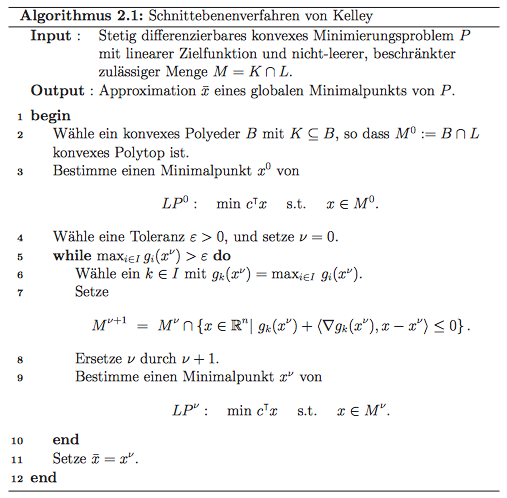
\includegraphics[scale=0.55]{img/vl-alg-21}
\end{figure*}

Es ist klar, dass Algorithmus 2.1 eine Folge $(x^\nu)$ erzeugt, die sich $M$ von außen nähert. Damit das Verfahren für eine beliebige Toleranz $\epsilon > 0$ nach endlich vielen Schritten abbricht, muss man noch ausschließen, dass die Folge $(x^\nu)$ einen positiven Abstand zu $M$ behält.

\begin{satz}[2.7.1]
	Algorithmus 2.1 bricht nach endlich vielen Schritten ab.	
\end{satz}

\subsection*{Verfahren von Frank-Wolfe (1956)}

Das folgende Verfahren basiert auf einer grundlegend anderen Idee als Schnittebenenverfahren: es erzeugt eine Folge von zulässigen Iterierten $(x^\nu)$, bis $x^\nu$ eine Optimalitätsbedingung ($\epsilon$-genau) erfüllt, während das Schnittebenenverfahren von Kelley aus der Optimalität im Hilfsproblem die Optimalität im Originalproblem schließt, falls die Iterierte $x^\nu$ ($\epsilon$-genau) zulässig ist. ~\bigskip

Gegeben sei das Problem
	$$ P: \quad \min f(x) \text{ s.t. } x \in M $$
mit nicht-leerer und konvexer zulässiger Menge $M$ sowie konvexer Zielfunktion $f \in C^1(M, \R)$.

\begin{satz}[2.7.2, Varationsformulierung konvexer Probleme]
	Unter obigen Voraussetzungen an $f$ und $M$ gilt:
	\begin{enumerate}
		\item $\overline{x} \in \R^n$ ist genau dann globaler Minimalpunkt von $P$, wenn $\overline{x}$ globaler Minimalpunkt von folgendem ist
			$$ Q(\overline{x}): \quad \min_x \langle \nabla f(\overline{x}), x - \overline{x} \rangle \text{ s.t. } x \in M $$
		\item Es sei $\overline{x} \in M$. Dann besitzt $Q(\overline{x})$ den Optimalwert $v(\overline{x}) \leq 0$, und $\overline{x}$ ist globaler Minimalpunkt von $P$ genau dann, wenn $v(\overline{x}) = 0$ gilt.
	\end{enumerate}	
\end{satz}

Das Verfahren von Frank-Wolfe basiert auf der Lösung von Hilfsproblemen der Form $Q(\overline{x})$. Damit diese überhaupt lösbar sind, fordern wir im Folgenden, dass $M$ nicht nur nicht-leer und konvex, sondern auch kompakt ist. Ferner wird das Verfahren nur dann numerisch interessant sein, wenn sich die Probleme $Q(\overline{x})$ schnell lösen lassen (also nicht z.B. durch Anwendung des Schnittebenenverfahrens von Kelley für jedes Hilfsproblem). Dies wird später auf weitere Voraussetzungen an $M$ führen. ~\bigskip

Der algorithmische Ansatz ist nun wie folgt. Wähle zunächst einen Startpunkt $x^0 \in M$ und bestimme den Minimalwert $v^0$ von $Q^0 \coloneqq Q(x^0)$. Falls $v^0 = 0$, stopp, denn nach Satz 2.7.2b) ist $x^0$ globaler Minimalpunkt von $P$. Da es eher unwahrscheinlich ist, dass man mit $x^0$ sofort einen globalen Minimalpunkt gefunden hat, ist die entscheidende Frage, wie man im Fall $v^0 < 0$ weiter vorgeht. ~\bigskip

Dazu sei zu $v^0$ auch ein Minimalpunkt $y^0$ von $Q^0$ bestimmt. Wie im Beweis zu Satz 2.7.2a) ist die Suchrichtung  $d^0 \coloneqq y^0 - x^0$ dann eine zulässige Abstiegsrichtung für $f$ in $x^0$, einen zulässigen Punkt mit kleinerem Zielfunktionswert findet man also auf jeden Fall in der Form $x^0 + t d^0$ mit einem passenden (d.h. nicht zu großen) $t \in [0, 1]$. ~\bigskip

Zur \textbf{Schrittweitensteuerung} (also zur Wahl der Schrittweite $t$) geht man folgendermaßen vor: wähle $t^0$ als Minimalpunkt von $f(x^0 + t d^0)$ auf $[0, 1]$, d.h. löse das eindimensionale Problem

	$$ S(x^0, d^0): \quad \min_t \underbrace{f(x^0 + t d^0)}_{konvex~in~t} \text{ s.t. } 0 \leq t \leq 1.$$

Auch $S(x^0, d^0)$ muss zur numerischen Umsetzung schnell lösbar sein, oder man gibt sich mit einer Approximation an $t^0$ zufrieden. ~\bigskip

Setze nun als neue Iterierte $x^1 \coloneqq x^0 + t^0 d^0$ und löse $Q^1$ usw. Das Abbruch-kriterium muss wieder relaxiert werden. Abbildung 2.25 zeigt die ersten zwei Iterationen des Verfahrens an einem Beispiel.

\begin{figure*}[h!] \centering
	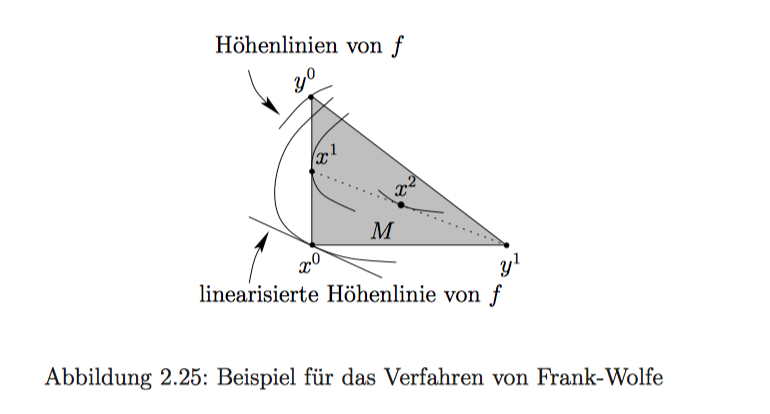
\includegraphics[scale=0.55]{img/vl-alg-23}
\end{figure*}


Das vollständige Verfahren ist in Algorithmus 2.2 angegeben. Um es numerisch sinnvoll einsetzen zu können, müssen die Hilfsprobleme $Q^\nu$ und $S(x^\nu, d^\nu)$ schnell lösbar sein.

\begin{figure*}[h!] \centering
	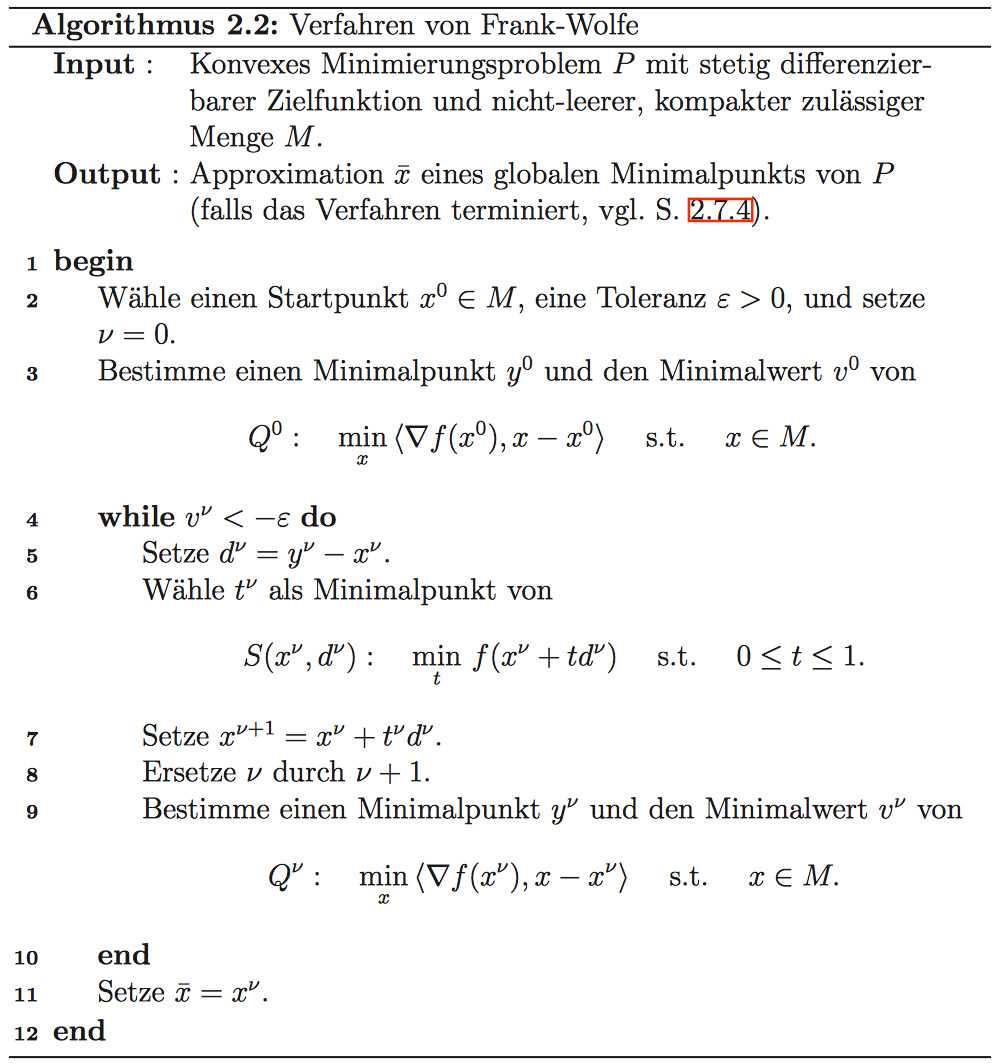
\includegraphics[scale=0.55]{img/vl-alg-22}
\end{figure*}

Für $Q^\nu$ sind dazu beispielsweise folgende Voraussetzungen geeignet:

\begin{itemize}
	\item falls $M$ ein konvexes Polytop ist (d.h. nur durch lineare Gleichungen und Ungleichungen beschrieben), dann ist $Q^\nu$ ein $LP$ und damit etwa per Simplex-Algorithmus lösbar, % todo simplex algorithmus
	\item falls $M$ eine Kugel ist, dann lässt sich $y^\nu$ sogar in geschlossener Form berechnen.
\end{itemize} % todo über geschlossene form nachdenken

Für $S(x^\nu, d^\nu)$ gilt: falls $f$ konvex-quadratisch ist, dann ist $t^\nu$ in geschlossener Form berechenbar. Daher wurde Algorithmus 2.2 im Jahr 1956 für konvex-quadratische Zielfunktionen mit linearen Nebenbedingungen formuliert.

\begin{uebung}[2.7.3]
	Mit $A = A^T \succ 0$ und $b \in \R^n$ sei $f(x) = \frac{1}{2} x^T A x + b^T x$. Geben Sie einen geschlossenen Ausdruck für den eindeutigen Minimalpunkt $t^\nu$ von $S(x^\nu, d^\nu)$ an.
\end{uebung} % todo alle uebungen

\begin{satz}[2.7.4]
	$\nabla f$ sei Lipschitz-stetig auf der nicht-leeren, konvexen und kompakten Menge $M$ (vgl. Def. 3.9.1). Dann bricht Algorithmus 2.2 nach endlich vielen Schritten ab.
\end{satz}

Da im Beweis zu Satz 2.7.4 nur die Effizienz der Schrittweitenfolge $(t^\nu)$ benutzt wird und nicht die Tatsache, dass die $t^\nu$ exakte globale Minimalpunkte von $S(x^\nu, d^\nu)$ sind, gilt die Konvergenzaussage auch noch, wenn $S(x^\nu, d^\nu)$ nur inexakt (z.B. per Armijoregel) gelöst wird. % todo Armijoregel

\subsection*{Primal-duale Innere-Punkte-Methoden}

Gegeben sei das konvexe $C^1$-Problem
	$$ P: \quad \min f(x) \text{ s.t. } g_i(x) \leq 0, ~ i \in I $$
mit beschränkter zulässiger Menge $M$ sowie
	$$ M_< \coloneqq \big\{ x \in \R^n ~|~g_i(x) < 0, ~ i \in I \big\} \neq 0 $$
(d.h. $M$ besitzt Slaterpunkte). Der Fall $J \neq 0$ kann auch betrachtet werden, wird es hier der Übersichtlichkeit halber aber nicht. ~\bigskip

Die primal-dualen Inneren-Punkte-Methoden basieren auf einem rein primalen Verfahren, nämlich dem \textbf{Barriereverfahren}. Seie Grundidee ist die Approximation von $P$ durch unrestringierte Probleme, wobei am Rand $bd M$ von $M$ eine \enquote{Barriere} errichtet wird, die die Zulässigkeit erzwingt. ~\bigskip

Zum Beispiel für das Problem 
	$$ \min -x \text{ s.t. } x \leq 0 $$
	ist $\beta(x) = -\log(-x)$ eine Barrierefunktion, d.h. $\beta \colon M_< \rightarrow \R$ und $\lim_{x^\nu \rightarrow x \in dbM} \beta(x^\nu) = + \infty$. ~\bigskip
	
Die Strategie des Barriereverfahrens besteht darin, die Nähe zum Rand von $M$ sukzesive weniger zu bestrafen, d.h. den Barriereparameter $t$ gegen null streben zu lassen und dabei Lösungen von
$$ \min_x B(t, x) \coloneqq -x -t\log(-x) $$
zu verfolgen. Für allgemine Zulässige Mengen von $P$ ist
$$ \beta(x) = -\sum_{i \in I} \log( -g_i(x)) $$
Barrierefunktion, und die Hilfprobleme 
$$ \min_x B(t, x) = f(x) - t\sum_{i \in I} \log(-g_i(x)) $$
sind für $t \rightarrow 0$ zu lösen.

\begin{satz}[2.7.5]
	Für alle $t > 0$ ist $B(t, x)$ konvex in $x$ und besitzt einen eindeutigen Minimalpunkt.
\end{satz}

Zu $t > 0$ bezeichne $x(t)$ den eindeutigen Minimalpunkt von $B(t,x)$. Die Menge
	$$ C_P = \big\{ x(t) ~|~t \in (0, \infty) \big\} $$
heißt \textbf{primaler zentraler Pfad} von $P$. Abbildung 2.28 illustriert primale zentrale Pfad für zwei lineare Optimierungsprobleme.

\begin{figure*}[h!] \centering
	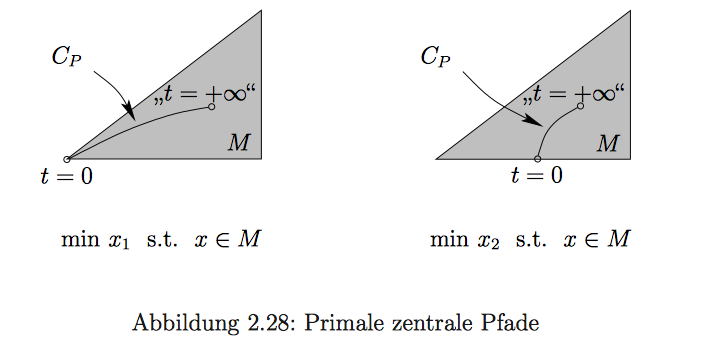
\includegraphics[scale=0.55]{img/vl-alg-24}
\end{figure*}

Unter schwachen Voraussetzungen ist $x^* = \lim_{t \rightarrow 0}x(t)$ ein globaler Minimalpunkt von $P$. Das Problem bei der numerischen Umsetzung dieses Ansatzes besteht darin, dass die Funktion $B(t, x)$ für $t \rightarrow 0+$ in der Nähe von $bdM$ stark gekrümmt, \enquote{numerisch geknickt} und damit schwer minimierbar ist. Dies spiegelt sich auch im Optimalitätskriterium wider: $x(t)$ ist die eindeutige Lösung von
	$$ 0= \nabla f(x) + \sum \left( - \frac{t}{g_i(x)} \right) \nabla g_i(x) $$
Für $x(t) \rightarrow x^* \in bdM$ gibt es mindestens ein $i \in I$ mit $g_i(x(t)) \rightarrow 0$, also ist $\lim_{t \rightarrow 0} \left( - \frac{t}{g_i(x(t))} \right)$ \enquote{vom Typ $\frac{0}{0}$} und die Optimalitätsbedingung damit für $t$ nahe null \enquote{schlecht konditioniert}. ~\bigskip

Als Ausweg macht man sich die Ähnlichkeit der obigen Optimalitätsbedingung zu den KKT-Bedingungen zu nutze und setzt für alle $t > 0$
$$ \lambda_i(t) \coloneqq - \frac{t}{g_i(x(t))}, ~ i \in I $$
Wegen $x(t) \in M_<$ gilt $g_i(x(t)) < 0$ für alle $i \in I$ und wegen $t > 0$ folgt daraus $\lambda_i(t) > 0$. Also ist $x(t)$ genau dann Minimalpunkt von $B(t, x)$, wenn ein $\lambda(t)$ existiert, so dass $(x(t), \lambda(t))$ das folgende System von Gleichungen und Ungleichungen löst:
	\begin{align*}
		\nabla f(x) + \sum_{i \in I} \lambda_i \nabla g_i(x) & = 0 \\
		\lambda_i g_i(x) & = -t \\
		-\lambda_i & > 0 \\
		g_i(x) & < 0, ~ i \in I
	\end{align*}
Dies ist gerade das KKT-System von $P$ mit durch $-t$ gestörter Komplementaritätsbedingung! Die Lösung $(x(t), \lambda(t))$ ist für alle $t > 0$ eindeutig, $x(t)$ ist \enquote{primal innerer Punkt}, und $\lambda(t)$ ist \enquote{dual innerer Punkt}. Die Menge
$$ C_{PD} = \big\{ (x(t), \lambda(t)) ~|~t \in (0, \infty) \big\} $$
heißt \textbf{primal-dualer zentraler Pfad} von $P$. ~\bigskip

Für $t \rightarrow 0+$ geht das gestörte in das ungestörte KKT-System über, d.h. bei Konvergenz $\lim_{t\rightarrow 0+} \left( x(t), \lambda(t) \right) = \left( x^*, \lambda^* \right)$ ist $x^*$ KKT-Punkt von $P$ mit Multiplikator $\lambda^*$ und damit globaler Minimalpunkt. Entscheidender Vorteil gegenüber dem Barriereverfahren ist, dass nun für $t \rightarrow 0+$ keine numerischen Probleme auftreten. ~\bigskip

Geschickte Implementierungen von primal-dualen Innere-Punkte-Methoden lösen die Hilfsprobleme für große $t$ nur grob, werden aber für $t \rightarrow 0+$ immer exakter. Außerdem bestimmen die Verfahren selbst die Anpassung von $t$. ~\bigskip

Dies kann sogar so geschehen, dass der Rechenaufwand zur Identifizierung einer $\epsilon$-genauen Lösung selbst im worst case nur \textit{polynomial in der Problemdimension} anwächst. Da dies insbesondere für lineare Optimierungsprobleme gilt, sind Innere-Punkte-Methoden in dieser Hinsicht dem Simplex-Algorithmus überlegen, der im worst case \textit{exponentiellen Rechenaufwand} besitzt. Bei hochdimensionalen Problemen lässt sich diese Überlegenheit tatsächlich beobachten, so dass kommerzielle Softwarepakete solche Probleme nicht per Simplex-Algorithmus lösen, sondern mit primal-dualen Innere-Punkte-Methoden. ~\bigskip

Von den in diesem Abschnitt behandelten speziell auf Konvexität zugeschnittenen Verfahren sind nur die primal-dualen Innere-Punkte-Methoden in der modernen Optimierung von praktischer Relevanz. Lösungsverfahren für allgemeine nichtlineare Optimierungsprobleme sind heute so weit entwickelt, dass sie dem Schnittebenenverfahren von Kelley und dem Verfahren von Frank-Wolfe im allgemeinen auch für konvexe Probleme überlegen sind. Es ist dennoch sinnvoll, diese Verfahren zu kennen, denn ihre Grundgedanken tauchen in veränderter Form zum Beispiel in der (gemischt-)ganzzahligen nichtlinearen Optimierung und bei der globalen Minimierung nicht-konvexer Funktionen wieder auf, dem Inhalt des nächsten Abschnitts.

\chapter{Nichtkonvexe Optimierung}

% Skript - Ende 			
\end{document}